\documentclass[11pt,a4paper]{article}
\usepackage[utf8]{inputenc}
\usepackage[margin=2.4cm]{geometry}
\usepackage{amsmath,amssymb,amsthm,mathtools,bm}
\usepackage{microtype}
\usepackage{booktabs,array,tabularx}
\usepackage{enumitem}
\usepackage{xcolor}
\usepackage{tikz}
\usetikzlibrary{arrows.meta,calc,positioning,shapes.geometric,shapes.symbols,decorations.pathreplacing,backgrounds,fit}
\usepackage{pgfplots}
\pgfplotsset{compat=1.16}
\usepackage[most]{tcolorbox}
\usepackage{listings}
\usepackage[hidelinks]{hyperref}
\usepackage{caption}
\captionsetup{font=small,labelfont=bf}
\setlength{\parindent}{0pt}
\setlength{\parskip}{5pt}

% ---------- notation ----------
\newcommand{\R}{\mathbb{R}}
\newcommand{\N}{\mathcal{N}}
\newcommand{\G}{\mathcal{G}}
\newcommand{\Lc}{\mathcal{L}}
\newcommand{\T}{^{\mathsf T}}
\newcommand{\abar}{\bar\alpha}
\DeclareMathOperator{\sigmoid}{sigmoid}
\DeclareMathOperator{\diag}{diag}
\DeclareMathOperator{\Tr}{tr}

% ---------- slide range tags ----------
\newcommand{\sr}[1]{\texorpdfstring{\emph{(#1)}}{(#1)}}

% ---------- theorem-like boxes (amsthm + tcolorbox) ----------
\theoremstyle{definition}
\newtheorem{definition}{Definition}[section]
\newtheorem{example}[definition]{Example}
\newtheoremstyle{algstyle}{\topsep}{\topsep}{\normalfont}{}{\bfseries}{.}{\newline}{}
\theoremstyle{algstyle}
\newtheorem{algorithm}[definition]{Algorithm}
\theoremstyle{plain}
\newtheorem{lemma}[definition]{Lemma}
\newtheorem{theorem}[definition]{Theorem}
\newtheorem{proposition}[definition]{Proposition}
\newtheorem{corollary}[definition]{Corollary}
\theoremstyle{remark}
\newtheorem{remark}[definition]{Remark}

\tcbset{thm/.style={enhanced,breakable,boxrule=0.6pt,arc=2pt,left=7pt,right=7pt,top=5pt,bottom=5pt,before skip=9pt,after skip=7pt}}
\tcolorboxenvironment{definition}{thm,colback=teal!5,colframe=teal!60!black}
\tcolorboxenvironment{lemma}{thm,colback=violet!5,colframe=violet!60!black}
\tcolorboxenvironment{theorem}{thm,colback=red!4,colframe=red!60!black}
\tcolorboxenvironment{proposition}{thm,colback=violet!5,colframe=violet!60!black}
\tcolorboxenvironment{corollary}{thm,colback=violet!5,colframe=violet!60!black}
\tcolorboxenvironment{example}{thm,colback=orange!6,colframe=orange!80!black}
\tcolorboxenvironment{algorithm}{thm,colback=gray!6,colframe=black!60}

\newtcolorbox{intuition}{enhanced,breakable,colback=blue!5,colframe=blue!60!black,
  fonttitle=\bfseries,title={Intuition},boxrule=0.5pt,arc=2pt,
  left=7pt,right=7pt,top=4pt,bottom=4pt,before skip=7pt,after skip=10pt}

% ---------- code listings ----------
\lstdefinestyle{py}{language=Python,basicstyle=\ttfamily\small,keywordstyle=\color{red!60!black}\bfseries,
  commentstyle=\color{gray}\itshape,columns=fullflexible,keepspaces=true,showstringspaces=false,
  breaklines=true,xleftmargin=2pt}
\lstset{style=py}

% ---------- placeholder for images to copy from the slides ----------
\newcommand{\slideimage}[3][3.8cm]{%
\begin{figure}[htbp]\centering
\begin{tikzpicture}
\draw[dashed,thick,gray!70,fill=gray!7] (0,0) rectangle (0.86\linewidth,#1);
\node[align=center,text=gray!70!black] at (0.43\linewidth,#1/2) {\textbf{[ insert image here ]}\\ taken from \textbf{slide #2}};
\end{tikzpicture}
\caption{#3}
\end{figure}}

% ---------- TikZ helpers ----------
\newcommand{\eye}[2]{\begin{scope}[shift={(#1,#2)}]
  \draw[thick,fill=white] (0,0) to[bend left=45] (0.7,0) to[bend left=45] (0,0);
  \fill[blue!45] (0.35,0) circle (0.09);\end{scope}}
% fuzzy Gaussian blob: x y rx ry angle colour
\newcommand{\blob}[6]{\begin{scope}[shift={(#1,#2)},rotate=#5]
  \shade[inner color=#6,outer color=#6!4] (0,0) ellipse (#3 and #4);\end{scope}}

\title{\textbf{Foundations of Spatial AI}\\[3pt]
Lecture 10 --- Differentiable Primitive Rendering\\[6pt]\large Detailed lecture notes}
\author{Based on the slides by Emanuele Giacomini and Luca Di Giammarino\\ Sapienza University of Rome}
\date{October 26, 2026}

\begin{document}
\maketitle
\tableofcontents

\bigskip
\begin{tcolorbox}[colback=gray!5,colframe=gray!50,boxrule=0.4pt,arc=2pt]
\textbf{How to read these notes.} Section and subsection titles follow the slide titles, and each carries its slide range. No companion book chapter was supplied, so the formal material (definitions, lemmas, proofs, derivations) was added from the standard sources the slides cite: Ravi et al.\ (PyTorch3D), Liu et al.\ (Soft Rasterizer), Zwicker et al.\ (EWA splatting), Kerbl et al.\ (3D Gaussian Splatting) and Huang et al.\ (2D Gaussian Splatting). Statements that go beyond the slides are labelled as such. Dashed boxes mark photos or screenshots to be copied from the indicated slide.
\end{tcolorbox}

\paragraph{Notation.} The slides reuse a few symbols in different sections; the context fixes the meaning.
\begin{center}
\small
\begin{tabular}{@{}p{3.6cm}p{11.3cm}@{}}
\toprule
Symbol & Meaning \\ \midrule
$\bm x_0,\ \bm\omega,\ \lambda$ & ray origin, unit direction, distance along the ray \\
$\bm v_1,\bm v_2,\bm v_3$ & triangle vertices; $(\alpha,\beta)$ barycentric coordinates (mesh sections) \\
$\bm c,\ \bm c_k$ & RGB colour of a pixel / of primitive $k$ \\
$m,\ \sigma,\ \gamma$ & soft mask, mask sharpness, depth-weighting temperature (soft meshes) \\
$\bm\mu,\ \bm p,\ \bm\Sigma$ & mean (position) and covariance of a Gaussian \\
$\bm R,\ \bm S$ & rotation and diagonal scale matrix, $\bm\Sigma=\bm R\bm S\bm S\T\bm R\T$ \\
$\alpha,\ \abar_k$ & opacity of a Gaussian / its opacity at a given pixel (Gaussian sections) \\
$T_k,\ w_k$ & transmittance in front of primitive $k$, blending weight \\
$\bm W,\ \bm t,\ \bm K$ & world$\to$camera rotation, translation, camera intrinsics \\
$\pi,\ \bm J$ & projection function, its Jacobian at the Gaussian mean \\
\bottomrule
\end{tabular}
\end{center}
\newpage
%=====================================================================
\section{Differentiable Primitive Rendering \sr{slides 1--7}}
%=====================================================================
The question of this lecture is how to render a scene made of \emph{primitives} (triangles, Gaussians, voxels, \dots) so that the image is a differentiable function of the primitive parameters. With such a renderer we can recover the scene by gradient descent on an image loss.

\subsection{Recap: Rendering Volumes \sr{slide 3}}
Volume rendering has two steps: (1) draw samples along the ray, (2) aggregate their contributions.

\begin{definition}[Discrete volume rendering]
Let a ray $\bm r(t)=\bm x_0+t\bm\omega$ be sampled at $t_1<\dots<t_N$ with spacings $\delta_i$, densities $\sigma_i$ and colours $\bm c_i$. Then
\[
\bm c=\sum_{i=1}^{N}T_i\,\alpha_i\,\bm c_i,\qquad
\alpha_i=1-e^{-\sigma_i\delta_i},\qquad
T_i=\prod_{j<i}(1-\alpha_j).
\]
\end{definition}

\begin{intuition}
$T_i$ is the fraction of light that survives up to sample $i$, and $\alpha_i$ is the share that sample $i$ absorbs and returns as its own colour. Everything in this lecture is a variation of this ``front-to-back'' bookkeeping. The only thing that changes is \emph{where} the contributions come from.
\end{intuition}

\begin{figure}[htbp]
\centering
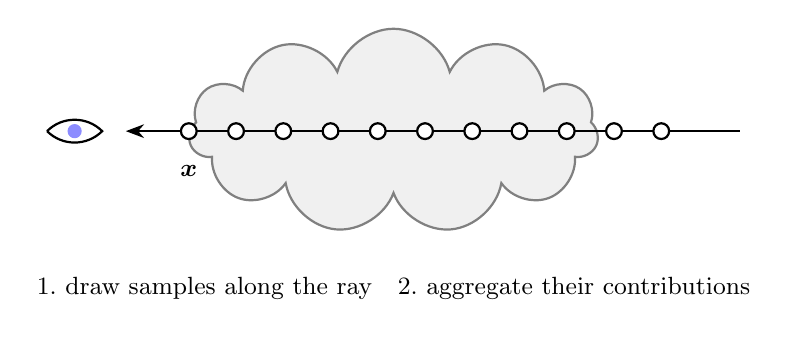
\begin{tikzpicture}[x=1cm,y=1cm]
\node[cloud,cloud puffs=11,draw=gray,thick,fill=gray!12,minimum width=5.2cm,minimum height=2.6cm] at (3.6,0) {};
\eye{-0.8}{0}
\draw[-{Stealth},thick] (8.0,0) -- (0.2,0);
\foreach \x in {1.0,1.6,2.2,2.8,3.4,4.0,4.6,5.2,5.8,6.4,7.0}{\draw[fill=white,thick] (\x,0) circle (0.1);}
\node[font=\small] at (1.0,-0.5) {$\bm x$};
\node[align=center,font=\small] at (3.6,-2.0) {1.\ draw samples along the ray\quad 2.\ aggregate their contributions};
\end{tikzpicture}
\caption{Volume rendering: samples are drawn along the ray through a volume and then aggregated.}
\end{figure}

\subsection{Rendering Primitives \sr{slides 4--6}}
\textbf{Gaussians (slide 4).} The same two steps work for primitives such as Gaussians: sample along the ray, aggregate whatever the samples hit.

\textbf{Triangles/meshes (slide 5).} Here step 1 is \emph{wasteful}: we know exactly where the primitives are, so most samples fall in empty space.

\textbf{The primitive view (slide 6).} Replace sampling by a direct query:
\begin{enumerate}[nosep]
\item \textbf{Find the primitives that affect the ray/pixel;}
\item \textbf{aggregate their contributions} to render the pixel.
\end{enumerate}

\begin{definition}[Primitive-based rendering]
A scene is a set of primitives $\{\mathsf p_k\}$, each with a geometry and an appearance. For a ray $\bm r$ let $\mathcal P(\bm r)=\{k:\mathsf p_k\text{ affects }\bm r\}$ be the \emph{influence set}. The pixel value is $\bm c(\bm r)=\mathrm{Agg}\big(\{(\lambda_k,\bm c_k,\dots)\}_{k\in\mathcal P(\bm r)}\big)$, where $\lambda_k$ is the depth of primitive $k$ along the ray.
\end{definition}

\begin{intuition}
The two design questions of the lecture are: how to compute $\mathcal P(\bm r)$ \emph{efficiently} (ray casting, then rasterization), and how to choose $\mathrm{Agg}$ so that the result is \emph{differentiable}.
\end{intuition}

\begin{figure}[htbp]
\centering
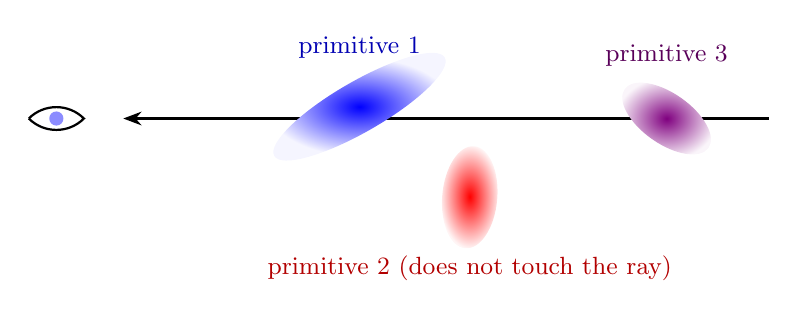
\begin{tikzpicture}
\eye{-1.2}{0}
\draw[-{Stealth},thick] (8.2,0) -- (0,0);
\blob{3.0}{0.15}{1.25}{0.32}{30}{blue}
\blob{4.4}{-1.0}{0.35}{0.65}{-5}{red}
\blob{6.9}{0.0}{0.65}{0.32}{-35}{violet}
\node[font=\small,blue!70!black] at (3.0,0.9) {primitive 1};
\node[font=\small,red!70!black] at (4.4,-1.9) {primitive 2 (does not touch the ray)};
\node[font=\small,violet!70!black] at (6.9,0.8) {primitive 3};
\end{tikzpicture}
\caption{Only primitives 1 and 3 are in the influence set $\mathcal P(\bm r)$ of this ray; primitive 2 is not.}
\end{figure}

\subsection{Today's Goals \sr{slide 7}}
\begin{enumerate}[nosep]
\item (Differentiable) mesh rendering via ray tracing.
\item From ray tracing to rasterization.
\item 3D Gaussian Splatting in detail: projection, tile rasterizer, optimization.
\end{enumerate}

%=====================================================================
\section{Mesh Rendering via Ray-casting \sr{slides 8--13}}
%=====================================================================
\subsection{Mesh Rendering via Ray-casting \sr{slide 8}}
For each pixel we cast a ray and (1) identify the \emph{closest} intersecting triangle, then (2) compute the appearance at the intersection point. Note that a \emph{mesh} is equivalent to a \emph{triangle set} for this algorithm: connectivity plays no role.

\slideimage[4.2cm]{8}{Ray cast from a pixel of the image plane through the cow mesh, hitting the closest triangle (red dot on the image plane, red arrow reaching the surface).}

\subsection{Mesh Rendering: Ray-Triangle Intersection \sr{slide 9}}
\begin{definition}[Barycentric coordinates]
Given a triangle $(\bm v_1,\bm v_2,\bm v_3)$, every point of its plane is written $\bm p=\alpha\bm v_1+\beta\bm v_2+(1-\alpha-\beta)\bm v_3$. The pair $(\alpha,\beta)$ are the barycentric coordinates of $\bm p$. The point lies inside the triangle iff $\alpha,\beta,1-\alpha-\beta\in(0,1)$.
\end{definition}

For a ray $(\bm x_0,\bm\omega)$ we need the point that is both on the ray and in the triangle plane:
\[
\bm p=\bm x_0+\lambda\bm\omega=\alpha\bm v_1+\beta\bm v_2+(1-\alpha-\beta)\bm v_3 .
\]
This is a linear system in $(\alpha,\beta,\lambda)$.

\begin{proposition}[Closed-form ray--triangle intersection]\label{prop:mt}
Let $\bm e_1=\bm v_1-\bm v_3$, $\bm e_2=\bm v_2-\bm v_3$, $\bm s=\bm x_0-\bm v_3$, and
$\bm h=\bm\omega\times\bm e_2$, $a=\bm e_1\cdot\bm h$, $\bm q=\bm s\times\bm e_1$. If $a\neq0$ (the ray is not parallel to the triangle),
\[
\alpha=\frac{\bm s\cdot\bm h}{a},\qquad
\beta=\frac{\bm\omega\cdot\bm q}{a},\qquad
\lambda=\frac{\bm e_2\cdot\bm q}{a}.
\]
\end{proposition}
\begin{proof}
Subtracting $\bm v_3$ from both sides gives $\alpha\bm e_1+\beta\bm e_2-\lambda\bm\omega=\bm s$, i.e.\ $[\bm e_1\ \bm e_2\ {-\bm\omega}]\,(\alpha,\beta,\lambda)\T=\bm s$. By Cramer's rule with $D=\det[\bm e_1\ \bm e_2\ {-\bm\omega}]=-\bm\omega\cdot(\bm e_1\times\bm e_2)$, and the cyclic invariance of the scalar triple product, one finds $D=-a$ and
$\alpha=\det[\bm s\ \bm e_2\ {-\bm\omega}]/D=\bm s\cdot\bm h/a$,
$\beta=\det[\bm e_1\ \bm s\ {-\bm\omega}]/D=\bm\omega\cdot\bm q/a$,
$\lambda=\det[\bm e_1\ \bm e_2\ \bm s]/D=\bm e_2\cdot\bm q/a$.
\end{proof}

\begin{intuition}
Think of two questions answered at once: ``where does the ray pierce the plane of the triangle?'' (that is $\lambda=-\bm s\cdot\bm n/\bm\omega\cdot\bm n$ with $\bm n=\bm e_1\times\bm e_2$) and ``where is that point expressed in the triangle's own $(\alpha,\beta)$ frame?''. Every ingredient is a smooth function of the vertices, which is why $(\alpha,\beta,\lambda)$ will turn out to be differentiable w.r.t.\ vertex positions.
\end{intuition}

\begin{figure}[htbp]
\centering
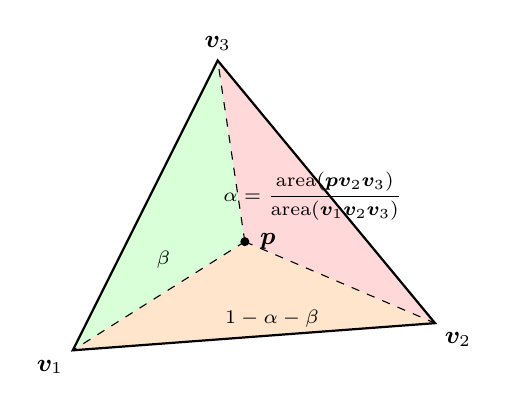
\begin{tikzpicture}[scale=1.15]
\coordinate (v1) at (0,0); \coordinate (v2) at (4,0.3); \coordinate (v3) at (1.6,3.2);
\coordinate (p) at (1.9,1.2);
\fill[blue!8] (v1)--(v2)--(v3)--cycle;
\fill[red!15] (p)--(v2)--(v3)--cycle;
\fill[green!15] (p)--(v1)--(v3)--cycle;
\fill[orange!20] (p)--(v1)--(v2)--cycle;
\draw[thick] (v1)--(v2)--(v3)--cycle;
\draw[dashed] (p)--(v1); \draw[dashed] (p)--(v2); \draw[dashed] (p)--(v3);
\fill (p) circle (0.05) node[right=2pt,font=\small] {$\bm p$};
\node[below left,font=\small] at (v1) {$\bm v_1$};
\node[below right,font=\small] at (v2) {$\bm v_2$};
\node[above,font=\small] at (v3) {$\bm v_3$};
\node[font=\scriptsize,align=center] at (2.65,1.7) {$\alpha=\dfrac{\text{area}(\bm p\bm v_2\bm v_3)}{\text{area}(\bm v_1\bm v_2\bm v_3)}$};
\node[font=\scriptsize,align=center] at (1.0,1.0) {$\beta$};
\node[font=\scriptsize,align=center] at (2.2,0.35) {$1-\alpha-\beta$};
\end{tikzpicture}
\caption{Barycentric coordinates as area ratios: the weight of a vertex is the relative area of the sub-triangle \emph{opposite} to it ($\beta$ is the area of $\bm p\bm v_1\bm v_3$, $1-\alpha-\beta$ the area of $\bm p\bm v_1\bm v_2$, both over the total).}
\end{figure}

\subsection{Mesh Rendering: Ray-Mesh Intersection \sr{slide 10}}
\begin{algorithm}[Closest intersecting triangle]
\begin{lstlisting}
def mesh_ray_intersection(mesh, ray):
    lam_min = inf
    intersection = None
    for triangle in mesh:
        (alpha, beta, lam) = intersect(ray, triangle)
        # inside test: 0 < alpha, beta, (1-alpha-beta) < 1
        if inside(alpha, beta) and 0 < lam < lam_min:
            lam_min = lam
            intersection = (triangle, (alpha, beta))
    return intersection
\end{lstlisting}
\end{algorithm}

\begin{remark}
The slide's code is explicitly ``rough pseudo-code''. It does not update \texttt{lam\_min}, which a working version must do, otherwise the \emph{closest} hit is not guaranteed. The cost is one intersection test per triangle \emph{per ray}.
\end{remark}

\subsection{Mesh Rendering \sr{slide 11}}
The two steps are two maps:
\[
\text{(1)}\ \ \text{mesh},\text{ray}\ \to\ \text{triangle},(\alpha,\beta)
\qquad
\text{(2)}\ \ \text{triangle},(\alpha,\beta)\ \to\ \bm c\in\R^3 .
\]

\subsection{Mesh Rendering: Appearance \sr{slide 12}}
\begin{definition}[Per-vertex colour and texture atlas]
\textbf{(a) Per-vertex colour:} each vertex carries a colour, $(\bm v_1,\bm v_2,\bm v_3)\to(\bm c_1,\bm c_2,\bm c_3)$, and
$\bm c=\alpha\bm c_1+\beta\bm c_2+(1-\alpha-\beta)\bm c_3$.
\textbf{(b) Texture atlas:} each triangle owns a $C\times C$ texture image and $\bm c=\text{bilinear\_sample}(\text{atlas},[\alpha,\beta])$.
\end{definition}
Appearance can be extended to lighting-dependent shading, using the albedo as stored texture together with the surface normals.

\begin{example}
Let $\bm c_1=(1,0,0)$, $\bm c_2=(0,1,0)$, $\bm c_3=(0,0,1)$ and $(\alpha,\beta)=(0.2,0.5)$. Then $\bm c=0.2\,\bm c_1+0.5\,\bm c_2+0.3\,\bm c_3=(0.2,0.5,0.3)$.
\end{example}

\begin{intuition}
Per-vertex colour is a smooth ``gradient'' blended over the triangle (cheap, low resolution). A texture atlas spends memory to store detail inside each face. In both cases the colour is a \emph{linear/bilinear} function of $(\alpha,\beta)$, hence trivially differentiable w.r.t.\ the barycentric coordinates.
\end{intuition}

\subsection{Mesh Rendering (differentiable?) \sr{slide 13}}
Step 1 gives $(\alpha,\beta)$ that are differentiable w.r.t.\ the mesh vertex positions (Proposition~\ref{prop:mt}); step 2 gives a colour differentiable w.r.t.\ the barycentric coordinates. The slide asks ``Is this differentiable?'' and answers: \emph{well, sort of\dots} The next section shows exactly where it fails.

%=====================================================================
\section{Mesh Rendering: Differentiability \sr{slide 14}}
%=====================================================================
The rendered colour \emph{is} differentiable w.r.t.\ the vertex positions of the visible triangle. For example, we can make the colour more red by changing the position of the triangle (it changes which part of the colour gradient lands on the pixel). Two things are not differentiable:
\begin{enumerate}[nosep]
\item rendering is discontinuous w.r.t.\ \textbf{occlusion/dis-occlusion};
\item rendering is discontinuous w.r.t.\ \textbf{depth ordering}.
\end{enumerate}

\begin{proposition}[Hard rendering is piecewise smooth]
Let $k^\star(\theta)=\arg\min_{k\,:\,\text{ray hits }k}\lambda_k(\theta)$ be the visible triangle for scene parameters $\theta$. The pixel value is $\bm c(\theta)=\bm c_{k^\star(\theta)}(\theta)$. On every region of parameter space where $k^\star$ is constant, $\bm c$ is smooth. Across a boundary where the visible triangle changes, $\bm c$ jumps. Consequently the gradient is either undefined at the jump or carries no information about it.
\end{proposition}

\begin{figure}[htbp]
\centering
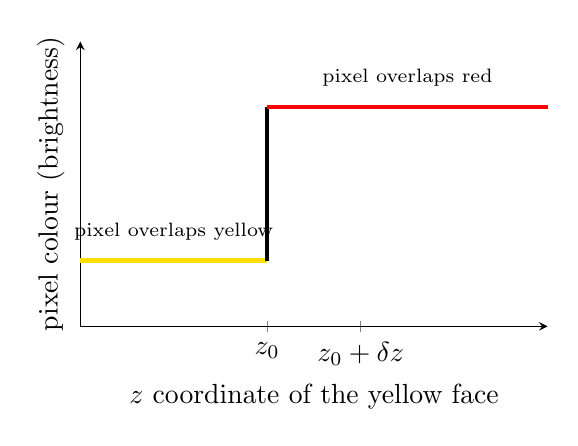
\begin{tikzpicture}
\begin{axis}[width=0.62\linewidth,height=5.2cm,axis lines=left,xlabel={$z$ coordinate of the yellow face},ylabel={pixel colour (brightness)},
 xmin=0,xmax=10,ymin=0,ymax=1.3,xtick={4,6},xticklabels={$z_0$,$z_0+\delta z$},ytick=\empty,clip=false]
\draw[yellow!80!orange,ultra thick] (axis cs:0,0.3) -- (axis cs:4,0.3);
\draw[black,ultra thick] (axis cs:4,0.3) -- (axis cs:4,1.0);
\draw[red,ultra thick] (axis cs:4,1.0) -- (axis cs:10,1.0);
\node[font=\scriptsize,anchor=south] at (axis cs:2,0.35) {pixel overlaps yellow};
\node[font=\scriptsize,anchor=south] at (axis cs:7,1.05) {pixel overlaps red};
\end{axis}
\end{tikzpicture}
\caption{Depth-ordering discontinuity (redrawn from the diagram on slide 14): as the yellow face is shifted behind the red one, the pixel colour jumps from yellow to red at a single $z$. The derivative is $0$ almost everywhere and undefined at the jump.}
\end{figure}

\slideimage[3.4cm]{14}{Original 3D sketch: shifting the yellow triangle by $+\delta z$ changes which face the pixel overlaps (left), and the occlusion example with an orange and a purple triangle (right).}

\begin{intuition}
Imagine you are blindfolded and can only feel the slope of the image at your feet. If the pixel is currently yellow, the slope of ``colour vs.\ $z$'' is flat: nothing you can feel says ``pushing the yellow face back would make the pixel red''. Likewise an \emph{occluded} triangle has \emph{exactly zero} influence on the image, so it never receives a gradient telling it to move into view.
\end{intuition}

%=====================================================================
\section{Differentiable Mesh Rendering \sr{slides 15--20}}
%=====================================================================
The fix (Ravi et al., PyTorch3D, 2020; Liu et al., Soft Rasterizer, ICCV 2019) has two parts: (1) make triangles \emph{soft}, (2) aggregate from \emph{multiple} triangles.

\subsection{Make triangles `soft' \sr{slides 15--16}}
\begin{definition}[Soft triangle mask]
Let $\Delta$ be the signed distance, in pixel space, from the pixel to the triangle ($\Delta<0$ inside, $>0$ outside). The soft mask is
\[
m=\sigmoid\!\Big(\frac{-\Delta}{\sigma}\Big)=\frac{1}{1+e^{\Delta/\sigma}},
\]
with a manually defined cut-off (e.g.\ $10\sigma$) beyond which the mask is set to zero.
\end{definition}

\begin{figure}[htbp]
\centering
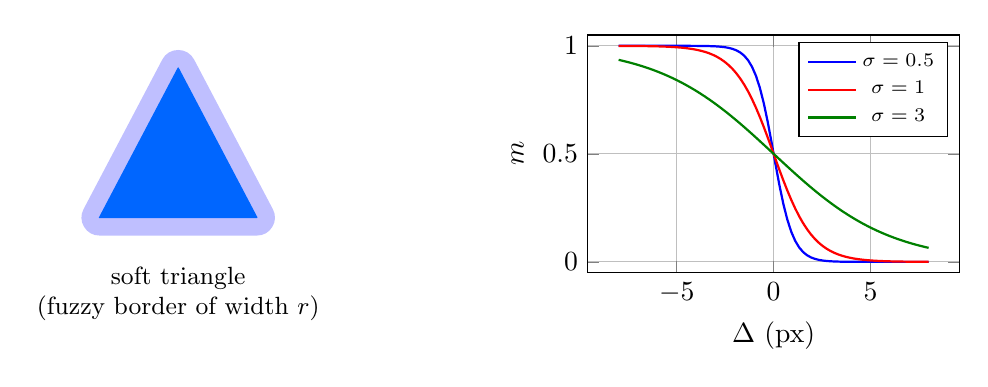
\begin{tikzpicture}
\begin{scope}
\draw[line width=13pt,line join=round,blue!25] (0,0)--(2,0)--(1,1.9)--cycle;
\draw[fill=blue!60!cyan,draw=blue!60!cyan,line join=round] (0,0)--(2,0)--(1,1.9)--cycle;
\node[font=\small,below,align=center] at (1,-0.5) {soft triangle\\(fuzzy border of width $r$)};
\end{scope}
\begin{scope}[xshift=6.2cm,yshift=-0.7cm]
\begin{axis}[width=0.52\linewidth,height=4.6cm,xlabel={$\Delta$ (px)},ylabel={$m$},domain=-8:8,samples=80,
 legend style={font=\scriptsize,at={(0.97,0.97)},anchor=north east},grid=both,ymin=-0.05,ymax=1.05]
\addplot[blue,thick]{1/(1+exp(x/0.5))}; \addlegendentry{$\sigma=0.5$}
\addplot[red,thick]{1/(1+exp(x/1))}; \addlegendentry{$\sigma=1$}
\addplot[green!50!black,thick]{1/(1+exp(x/3))}; \addlegendentry{$\sigma=3$}
\end{axis}
\end{scope}
\end{tikzpicture}
\caption{Left: a soft triangle has a fuzzy border of width $r$ (slide 15--16). Right: the mask $m=\sigmoid(-\Delta/\sigma)$ for several $\sigma$; $m=0.5$ exactly on the boundary.}
\end{figure}

\begin{proposition}[Properties of the soft mask]
(i) $m\to1$ deep inside and $m\to0$ far outside; $m=\tfrac12$ on the boundary. (ii) $\partial m/\partial\Delta=-m(1-m)/\sigma$ is non-zero for every pixel near the triangle. (iii) As $\sigma\to0$, $m$ converges to the hard indicator of the triangle.
\end{proposition}
\begin{proof}
(i)--(iii) follow from the shape of the logistic function; (ii) is its derivative $\sigma'(x)=\sigma(x)(1-\sigma(x))$ with the chain rule on $x=-\Delta/\sigma$.
\end{proof}

\begin{example}
With $\sigma=1$: a pixel 2 px \emph{outside} ($\Delta=2$) gets $m=\sigmoid(-2)=0.119$, while one 3 px \emph{inside} ($\Delta=-3$) gets $m=\sigmoid(3)=0.953$. With $\sigma=2$ the outside pixel gets $\sigmoid(-1)=0.269$: a larger $\sigma$ blurs the silhouette.
\end{example}

\begin{intuition}
A hard triangle is a cookie cutter: a pixel is either in or out. A soft triangle is a cookie with a fuzzy rim. A pixel just outside the rim still ``feels'' the triangle a little, and therefore the loss on that pixel can pull the triangle's vertices towards it. This is the gradient signal that hard rasterization lacks.
\end{intuition}

\subsection{Aggregate from multiple triangles \sr{slide 17}}
For each pixel:
\begin{enumerate}[nosep]
\item find the $K$ closest triangles that have a non-zero mask at the pixel (same code as for the single closest triangle);
\item weight each triangle by its mask and distance along the ray, $w_k\propto m_k\,e^{-\lambda_k/\gamma}$ (a small default weight $w_{bg}$ can model the background);
\item combine the per-triangle appearance, $\bm c=\sum_k w_k\bm c_k$.
\end{enumerate}

\begin{definition}[Soft blending of $K$ triangles]
With the weights normalised to sum to one,
\[
w_k=\frac{m_k\,e^{-\lambda_k/\gamma}}{\sum_{j=1}^{K}m_j\,e^{-\lambda_j/\gamma}+w_{bg}},\qquad
\bm c=\sum_{k=1}^{K}w_k\bm c_k+w_{bg}'\,\bm c_{bg},
\]
where $w_{bg}'=w_{bg}/(\sum_j m_je^{-\lambda_j/\gamma}+w_{bg})$ is the background's share.
\end{definition}

\begin{proposition}[Limits and gradient of soft blending]\label{prop:softblend}
(a) If $m_j>0$ and $\lambda_j<\lambda_k$ then $w_k/w_j=(m_k/m_j)\,e^{-(\lambda_k-\lambda_j)/\gamma}\to0$ as $\gamma\to0$: the closest triangle wins and we recover the hard z-buffer. (b) For fixed masks and no background, $\dfrac{\partial\bm c}{\partial\lambda_k}=-\dfrac{w_k}{\gamma}\,(\bm c_k-\bm c)$.
\end{proposition}
\begin{proof}
(a) is the ratio of two weights. (b) The weights are a softmax of $-\lambda_j/\gamma+\log m_j$, so $\partial w_j/\partial\lambda_k=-\tfrac1\gamma w_j(\delta_{jk}-w_k)$. Hence $\partial\bm c/\partial\lambda_k=\sum_j\bm c_j\,\partial w_j/\partial\lambda_k=-\tfrac1\gamma(w_k\bm c_k-w_k\sum_jw_j\bm c_j)$.
\end{proof}

\begin{example}
Two fully visible triangles ($m=1$) at depths $\lambda_1=1$, $\lambda_2=2$. For $\gamma=1$ the weights are $\propto e^{-1}=0.368$ and $e^{-2}=0.135$, i.e.\ $w=(0.731,0.269)$. For $\gamma=0.1$ the ratio is $e^{-10}\approx4.5\cdot10^{-5}$, so $w\approx(0.99995,0.00005)$: almost a hard z-buffer.
\end{example}

\begin{intuition}
The mask answers ``is this triangle over the pixel?'', the exponential answers ``how much does this one deserve to be seen, given how far it is?''. $\gamma$ is a temperature: large $\gamma$ lets triangles behind show through (semi-transparency, good gradients), small $\gamma$ is a crisp opaque rendering. By Proposition~\ref{prop:softblend}(b) even a partially hidden triangle ($w_k>0$) gets a gradient that nudges it towards or away from the camera, which fixes the depth-ordering problem of the previous section.
\end{intuition}

\subsection{Effect of $\gamma$ and $\sigma$, and an example \sr{slides 18--19}}
\slideimage[3.6cm]{18}{Cube rendered with standard rendering (left), with a larger $\gamma$ (middle: back faces show through) and with larger $\gamma$ and $\sigma$ (right: blurred silhouette). From Liu et al., ICCV 2019.}

\slideimage[5.0cm]{19}{Soft Rasterizer example: a mesh is optimised from an initialization towards a target image/silhouette (the red hand is the part that has to move); the right part shows intermediate optimisation results.}

\subsection{Differentiable Mesh Rendering via Ray tracing \sr{slide 20}}
\begin{enumerate}[nosep]
\item Identify the closest $K$ `softly' intersecting triangles (and the corresponding pixel-space SDF);
\item aggregate appearance using masks, depth-dependent weights, and per-triangle appearance.
\end{enumerate}

\begin{algorithm}[Ray-traced soft mesh rendering, slide 21 structure]
\begin{lstlisting}
def render(mesh, camera):
    ### Iterate over all pixels
    for pixel in camera.grid:
        ray = pixel2ray(camera, pixel)
        ### Iterate over all triangles
        for triangle in mesh:
            # Find current K closest intersecting triangles
        ### Iterate over triangles influencing this pixel
        for triangle in sorted_k_closest:
            # Aggregate appearance
\end{lstlisting}
\end{algorithm}

%=====================================================================
\section{From Ray tracing to Rasterization \sr{slides 21--25}}
%=====================================================================
\subsection{Redundant computation \sr{slide 21}}
In the code above, neighbouring pixels (two rays on the cow's nose) loop over the \emph{same} triangles and redo much of the same work. \textbf{Idea: iterate over triangles just once, and store which pixels they affect.}

\begin{proposition}[Cost of the two loop orders]
Let $P$ be the number of pixels, $N$ the number of primitives, $\bar f$ the average number of pixels a primitive's footprint covers and $K$ the number of triangles kept per pixel. Pixel-major (ray tracing) costs $\Theta(PN)$ intersection tests. Primitive-major (rasterization + blending) costs $\Theta(N\bar f)$ to fill the per-pixel structure plus $\Theta(PK)$ to blend.
\end{proposition}
\begin{example}
$P=10^6$ pixels, $N=10^6$ triangles, $\bar f=10$, $K=10$: pixel-major needs $10^{12}$ tests; primitive-major needs about $10^{7}+10^{7}=2\cdot10^{7}$ operations (ignoring the $\log K$ factor of buffer insertion), five orders of magnitude less.
\end{example}
\begin{intuition}
Instead of asking every pixel ``who is on top of you?'', we ask every triangle ``whom do you cover?''. A triangle is small, so it covers few pixels, and the answer is cheap. Ray tracing is a \emph{gather} (pixels pull), rasterization is a \emph{scatter} (primitives push).
\end{intuition}

\subsection{From Ray tracing to Rasterization \sr{slides 22--23}}
\begin{figure}[htbp]
\centering
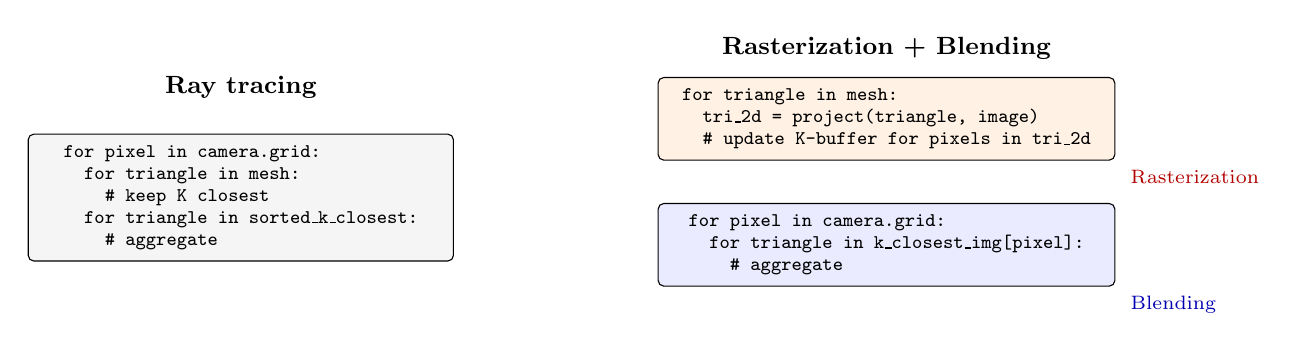
\begin{tikzpicture}[box/.style={draw,rounded corners=2pt,align=left,font=\scriptsize\ttfamily,inner sep=4pt,fill=white},lab/.style={font=\small\bfseries}]
\node[lab] at (0,2.6) {Ray tracing};
\node[box,fill=gray!8,minimum width=5.4cm,align=left] (a) at (0,1.2) {for pixel in camera.grid:\\\hspace*{1em}for triangle in mesh:\\\hspace*{2em}\# keep K closest\\\hspace*{1em}for triangle in sorted\_k\_closest:\\\hspace*{2em}\# aggregate};
\node[lab] at (8.2,3.1) {Rasterization + Blending};
\node[box,fill=orange!10,minimum width=5.8cm] (b) at (8.2,2.2) {for triangle in mesh:\\\hspace*{1em}tri\_2d = project(triangle, image)\\\hspace*{1em}\# update K-buffer for pixels in tri\_2d};
\node[box,fill=blue!8,minimum width=5.8cm] (c) at (8.2,0.6) {for pixel in camera.grid:\\\hspace*{1em}for triangle in k\_closest\_img[pixel]:\\\hspace*{2em}\# aggregate};
\node[font=\scriptsize,red!70!black,right=2pt of b.south east,anchor=north west] {Rasterization};
\node[font=\scriptsize,blue!70!black,right=2pt of c.south east,anchor=north west] {Blending};
\end{tikzpicture}
\caption{Swapping the loop order: the K closest triangles per pixel are found while iterating over triangles once, and the pixel loop only blends (slide 22).}
\end{figure}

\begin{algorithm}[Rasterization-based soft mesh rendering]
\begin{lstlisting}
def render(mesh, camera):
    ### some structure to store K triangles for each pixel
    sorted_k_closest_img = ...
    ### Iterate over all triangles   (Rasterization)
    for triangle in mesh:
        tri_2d = project(triangle, image)
        # Update closest_K_img for pixels within tri_2d
    ### Iterate over all pixels      (Blending + Shading)
    for pixel in camera.grid:
        for triangle in sorted_k_closest_img[pixel]:
            # Aggregate appearance
\end{lstlisting}
\end{algorithm}

On slide 23 the PyTorch3D renderer is drawn as the pipeline below.

\begin{figure}[htbp]
\centering
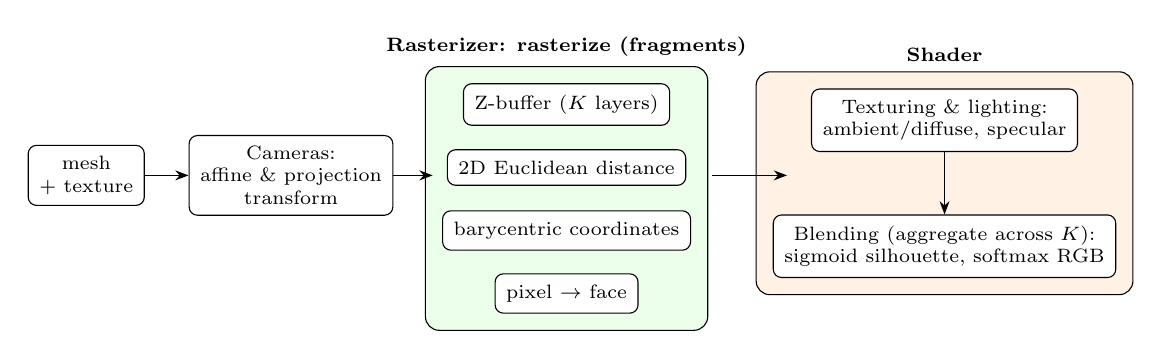
\begin{tikzpicture}[blk/.style={draw,rounded corners=3pt,align=center,font=\scriptsize,fill=white,inner sep=4pt},
 grp/.style={draw,rounded corners=5pt,fill=#1,inner sep=6pt}, >={Stealth}]
\node[blk] (mesh) at (0,0) {mesh\\+ texture};
\node[blk] (cam) at (2.6,0) {Cameras:\\affine \& projection\\transform};
\node[blk] (z) at (6.1,0.9) {Z-buffer ($K$ layers)};
\node[blk] (d) at (6.1,0.1) {2D Euclidean distance};
\node[blk] (b) at (6.1,-0.7) {barycentric coordinates};
\node[blk] (p) at (6.1,-1.5) {pixel $\to$ face};
\node[blk] (tex) at (10.9,0.7) {Texturing \& lighting:\\ambient/diffuse, specular};
\node[blk] (bl) at (10.9,-0.9) {Blending (aggregate across $K$):\\sigmoid silhouette, softmax RGB};
\begin{scope}[on background layer]
\node[grp=green!8,fit=(z)(d)(b)(p),label={[font=\scriptsize\bfseries]above:Rasterizer: rasterize (fragments)}] {};
\node[grp=orange!10,fit=(tex)(bl),label={[font=\scriptsize\bfseries]above:Shader}] {};
\end{scope}
\draw[->] (mesh)--(cam); \draw[->] (cam)--(4.4,0);
\draw[->] (7.95,0)--(8.9,0);
\draw[->] (tex)--(bl);
\end{tikzpicture}
\caption{The PyTorch3D renderer (Ravi et al., 2020), redrawn from slide 23: a rasterizer produces per-pixel fragments (depth, distance, barycentrics, face index, $K$ layers) and a shader textures, lights and blends them. The sigmoid silhouette is the soft mask $m$ and the softmax RGB is the depth-weighted combination above.}
\end{figure}

\subsection{Differentiable Primitive Rendering \sr{slides 24--25}}
The loop structure is independent of the primitive type:
\begin{algorithm}[Generic differentiable primitive rendering]
\begin{lstlisting}
def render(primitives, camera):
    # Initialize a rasterization data structure
    # (records influencing primitives for each pixel)
    for primitive in primitives:                 # Rasterization
        prim2d = project(primitive, camera)
        # Update rasterization data structure
    for pixel in camera.grid:                    # Blending
        # Aggregate appearance from influencing primitives
\end{lstlisting}
\end{algorithm}
For Gaussians (slide 25) the same code is instantiated with \texttt{gaussians}, projecting each one to a 2D Gaussian (\texttt{gauss2d}). To fill it in we must answer three questions: \emph{What is the representation of a 3D Gaussian? How to project to 2D and rasterize? How to model/aggregate appearance?}
%=====================================================================
\section{Differentiable Gaussian Rendering \sr{slides 26--38}}
%=====================================================================
\subsection{What is the representation of a 3D gaussian? \sr{slides 26--29}}
\slideimage[4.6cm]{26}{A real scene (forest, left) and a view of the same scene where the individual Gaussians are visible as flat shaded blobs (right).}

\subsubsection{Gaussian primitive \sr{slide 27}}
\begin{definition}[3D Gaussian primitive]
A Gaussian primitive is the tuple $(\bm p,\bm\Sigma,\alpha,\bm c)$ with density
\[
\G_{\bm\Sigma}(\bm x-\bm p)=\frac{1}{(2\pi)^{3/2}|\bm\Sigma|^{1/2}}\,
\exp\!\Big(-\tfrac12(\bm x-\bm p)\T\bm\Sigma^{-1}(\bm x-\bm p)\Big),
\]
an opacity $\alpha$, and a view-dependent colour $\bm c$ given by spherical-harmonics (SH) coefficients. The covariance is factorised into scale and rotation,
\[
\bm\Sigma=\bm R\bm S\bm S\T\bm R\T,\qquad \bm S=\diag(s_1,s_2,s_3).
\]
\end{definition}

The level sets $(\bm x-\bm p)\T\bm\Sigma^{-1}(\bm x-\bm p)=\text{const}$ are ellipsoids whose axes are the columns of $\bm R$ with semi-axis lengths proportional to $s_i$.

\begin{figure}[htbp]
\centering
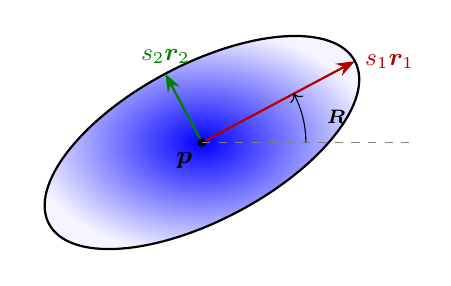
\begin{tikzpicture}[scale=1.1]
\begin{scope}[rotate=28]
\blob{0}{0}{2.0}{0.9}{0}{blue}
\draw[thick] (0,0) ellipse (2.0 and 0.9);
\draw[-{Stealth},thick,red!70!black] (0,0)--(2.0,0) node[right,font=\small] {$s_1\bm r_1$};
\draw[-{Stealth},thick,green!50!black] (0,0)--(0,0.9) node[above,font=\small] {$s_2\bm r_2$};
\end{scope}
\fill (0,0) circle (0.05) node[below left,font=\small] {$\bm p$};
\draw[gray,dashed] (0,0)--(2.4,0); \draw[->] (1.2,0) arc (0:28:1.2); \node[font=\scriptsize] at (1.55,0.3) {$\bm R$};
\end{tikzpicture}
\caption{A 2D slice of a Gaussian: position $\bm p$, principal axes $\bm r_i$ (columns of $\bm R$) and scales $s_i$.}
\end{figure}

\begin{remark}[Normalisation, beyond the slides]
The slide writes the normalised density (with the factor $1/((2\pi)^{3/2}|\bm\Sigma|^{1/2})$). In the reference 3DGS implementation (Kerbl et al.) the opacity $\alpha$ multiplies the \emph{unnormalised} exponential, so $\alpha$ is the peak opacity of the primitive. The code on slide 37 does exactly this.
\end{remark}

\begin{intuition}
A 3D Gaussian is a soft ellipsoidal ``cloud of paint'': densest at the centre, fading smoothly outwards, stretched along the directions of $\bm R$. Because the fall-off is smooth and infinitely differentiable, small changes of $\bm p,\bm s,\bm R,\alpha$ change the image smoothly, which is what we need for gradients.
\end{intuition}

\subsubsection{What Each Gaussian Stores \sr{slide 28}}
\begin{center}
\begin{tabular}{@{}lll@{}}
\toprule
Parameter & Symbol & Floats \\ \midrule
Position & $\bm\mu$ & 3 \\
Scale & $\bm s$ & 3 \\
Rotation (quaternion) & $\bm q$ & 4 \\
Opacity & $\alpha$ & 1 \\
Colour, SH degree 3 & & $48$ \\ \midrule
\textbf{Total} & & \textbf{59} \\ \bottomrule
\end{tabular}
\end{center}
SH of degree 3 has $(3+1)^2=16$ coefficients per colour channel, i.e.\ $16\times3=48$ floats.

\begin{example}
About $3\cdot10^{6}$ Gaussians per scene, at $59\times4=236$ bytes each, give $\approx708$~MB, i.e.\ the ``$\sim$700~MB'' on the slide (consistent with the 734~MB of the results table later).
\end{example}

\subsubsection{Why Not Optimize the Covariance Directly? \sr{slide 29}}
A gradient step on $\bm\Sigma$ can destroy its validity: the slide's example moves $\diag(1,0.01,1)$ by $-\eta\nabla\Lc$ to $\diag(1,-0.02,1)$, a \emph{negative variance}, which is not a Gaussian at all.

\begin{proposition}[Factorised covariance is always PSD]
For any rotation $\bm R$ and any real $\bm S=\diag(s_1,s_2,s_3)$, $\bm\Sigma=\bm R\bm S\bm S\T\bm R\T=(\bm R\bm S)(\bm R\bm S)\T$ is symmetric positive semi-definite, since
$\bm x\T\bm\Sigma\bm x=\|\bm S\T\bm R\T\bm x\|^2\ge0$. Conversely, every symmetric positive definite $\bm\Sigma$ has such a factorisation (spectral theorem: $\bm\Sigma=\bm Q\bm\Lambda\bm Q\T$, take $\bm R=\bm Q$, $\bm S=\bm\Lambda^{1/2}$).
\end{proposition}

\begin{intuition}
Optimising $\bm\Sigma$ directly is like steering a car by moving the wheels' bolts around: nothing prevents an impossible configuration. Optimising $(\bm S,\bm R)$ instead is steering with the wheel: whatever you do, you still get a valid ellipsoid. In the example above the update on $s_2=0.1$ can make $s_2$ any real number, but $\Sigma_{22}=s_2^2$ is never negative.
\end{intuition}

\begin{remark}[Beyond the slides]
In the reference implementation the scale is stored in log-space (activation $\exp$) so that $s_i>0$, the rotation is a quaternion that is normalised before building $\bm R$, and opacity is stored before a sigmoid so that $\alpha\in(0,1)$. The colour is $\bm c(\bm d)=\sum_{\ell\le3}\sum_{m}k_{\ell m}Y_\ell^m(\bm d)$ for the viewing direction $\bm d$.
\end{remark}

\subsection{How to project to 2D and rasterize? \sr{slides 30--34}}
\subsubsection{World to camera \sr{slides 30--31}}
We use the camera extrinsics to transform each 3D Gaussian to the camera frame: $(\bm p,\bm R,\bm S)\to(\bm p',\bm R',\bm S)$.

\begin{lemma}[Affine maps keep Gaussians Gaussian]\label{lem:affine}
If $\bm x\sim\N(\bm\mu,\bm\Sigma)$ then $\bm A\bm x+\bm b\sim\N(\bm A\bm\mu+\bm b,\ \bm A\bm\Sigma\bm A\T)$.
\end{lemma}
\begin{proof}
The characteristic function of $\bm x$ is $\varphi(\bm t)=\exp(i\bm t\T\bm\mu-\tfrac12\bm t\T\bm\Sigma\bm t)$. For $\bm y=\bm A\bm x+\bm b$, $\varphi_y(\bm t)=e^{i\bm t\T\bm b}\varphi(\bm A\T\bm t)=\exp\big(i\bm t\T(\bm A\bm\mu+\bm b)-\tfrac12\bm t\T\bm A\bm\Sigma\bm A\T\bm t\big)$, which is the characteristic function of $\N(\bm A\bm\mu+\bm b,\bm A\bm\Sigma\bm A\T)$. Note that $\bm A$ need not be invertible.
\end{proof}

World$\to$camera is affine, so
\[
\bm\mu_c=\bm W\bm\mu+\bm t,\qquad\bm\Sigma_c=\bm W\bm\Sigma\bm W\T=(\bm W\bm R)\bm S\bm S\T(\bm W\bm R)\T,
\]
that is $\bm p'=\bm W\bm p+\bm t$, $\bm R'=\bm W\bm R$ and the scale is unchanged (slide 30).

\begin{figure}[htbp]
\centering
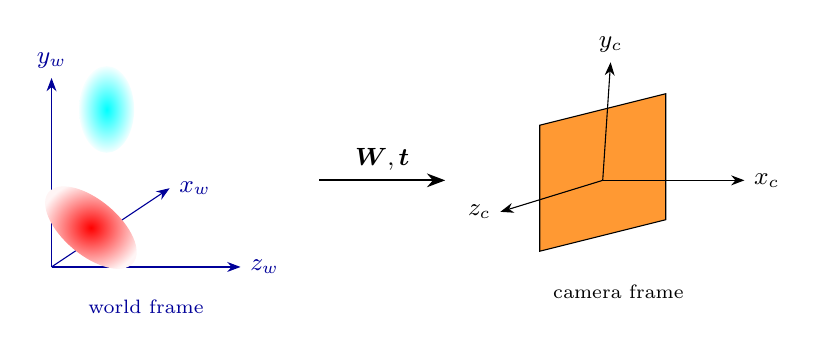
\begin{tikzpicture}[>={Stealth}]
\begin{scope}
\draw[->,blue!60!black] (0,0)--(2.4,0) node[right,font=\small] {$z_w$};
\draw[->,blue!60!black] (0,0)--(0,2.4) node[above,font=\small] {$y_w$};
\draw[->,blue!60!black] (0,0)--(1.5,1.0) node[right,font=\small] {$x_w$};
\blob{0.7}{2.0}{0.35}{0.55}{0}{cyan}
\blob{0.5}{0.5}{0.7}{0.35}{-40}{red}
\node[font=\scriptsize,blue!60!black,below] at (1.2,-0.3) {world frame};
\end{scope}
\draw[->,thick] (3.4,1.1)--(5.0,1.1) node[midway,above,font=\small] {$\bm W,\bm t$};
\begin{scope}[xshift=6.2cm]
\draw[fill=orange!80,draw=black] (0,0.2)--(1.6,0.6)--(1.6,2.2)--(0,1.8)--cycle;
\draw[->] (0.8,1.1)--(2.6,1.1) node[right,font=\small] {$x_c$};
\draw[->] (0.8,1.1)--(0.9,2.6) node[above,font=\small] {$y_c$};
\draw[->] (0.8,1.1)--(-0.5,0.7) node[left,font=\small] {$z_c$};
\node[font=\scriptsize,below] at (1.0,-0.1) {camera frame};
\end{scope}
\end{tikzpicture}
\caption{Gaussians are expressed in the camera frame by the affine map $(\bm W,\bm t)$ (slides 30--31).}
\end{figure}

\begin{intuition}
Changing the viewpoint does not change the cloud of paint; it only changes the coordinates in which we describe it. A rigid motion rotates the ellipsoid ($\bm R\to\bm W\bm R$) and moves its centre, nothing else.
\end{intuition}

\subsubsection{Projection to the image \sr{slides 32--33}}
Let $\pi$ map 3D points to pixels: $\pi(\bm x)=\bm u$ with $z\,(u,v,1)\T=\bm K\,(X,Y,Z)\T$. The 2D mean is $\bm\mu_{2D}=\pi(\bm\mu_{3D})$. \emph{What is the image-space projection of a 3D Gaussian?} It can be approximated as a 2D Gaussian (EWA Volume Splatting, Zwicker et al., 2001), with covariance
\[
\bm\Sigma_{2D}=\bm J\,\bm\Sigma_{3D}\,\bm J\T,\qquad\bm J=\frac{\partial\pi}{\partial\bm x}(\bm\mu_{3D}).
\]

The projection is \emph{not} affine: $\pi(\bm x_c)=\big(f_xX/Z+c_x,\ f_yY/Z+c_y\big)\T$ with $\bm x_c=(X,Y,Z)\T$.

\begin{theorem}[EWA: local affine approximation of the projection]\label{thm:ewa}
Let $\bm x_c\sim\N(\bm\mu_c,\bm\Sigma_c)$ with $\bm\Sigma_c=\bm W\bm\Sigma\bm W\T$. Linearising $\pi$ at the mean,
$\pi(\bm x_c)\approx\pi(\bm\mu_c)+\bm J(\bm x_c-\bm\mu_c)$, with
\[
\bm J=\left.\frac{\partial\pi}{\partial\bm x_c}\right|_{\bm\mu_c}=
\begin{bmatrix}f_x/Z&0&-f_xX/Z^2\\0&f_y/Z&-f_yY/Z^2\end{bmatrix}_{\bm\mu_c},
\]
the projected Gaussian is $\N(\bm\mu_{2D},\bm\Sigma_{2D})$ with $\bm\mu_{2D}=\pi(\bm\mu_c)$ and
$\bm\Sigma_{2D}=\bm J\bm W\bm\Sigma\bm W\T\bm J\T\in\R^{2\times2}$.
\end{theorem}
\begin{proof}
The linearisation is an affine map of $\bm x_c$ with linear part $\bm J$. Apply Lemma~\ref{lem:affine}. The derivatives are those of $f_xX/Z$ and $f_yY/Z$.
\end{proof}

\begin{example}
Take $f_x=f_y=500$, $(c_x,c_y)=(320,240)$, $\bm\mu_c=(0.2,-0.1,2.0)$ and $\bm\Sigma_c=\diag(0.01,0.01,0.04)$. Then $\bm\mu_{2D}=(500\cdot0.1+320,\ 500\cdot(-0.05)+240)=(370,215)$ and
$\bm J=\begin{bmatrix}250&0&-25\\0&250&12.5\end{bmatrix}$, so
\[
\bm\Sigma_{2D}=\begin{bmatrix}250^2\cdot0.01+25^2\cdot0.04&-25\cdot12.5\cdot0.04\\ \cdot&250^2\cdot0.01+12.5^2\cdot0.04\end{bmatrix}
=\begin{bmatrix}650&-12.5\\-12.5&631.25\end{bmatrix},
\]
i.e.\ a splat with standard deviation of about $25$ px. The depth uncertainty (0.04) leaks into the image through the off-axis entries of $\bm J$.
\end{example}

\begin{figure}[htbp]
\centering
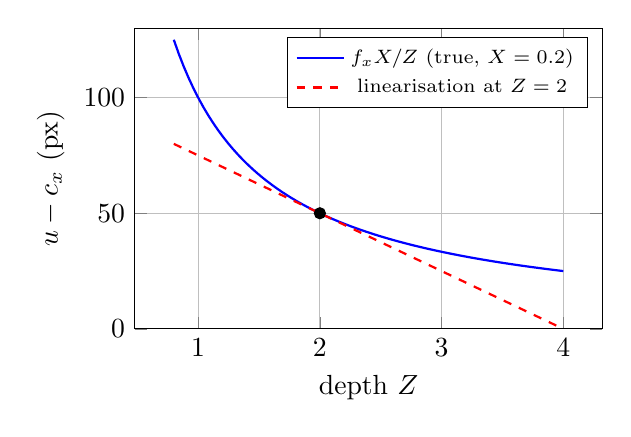
\begin{tikzpicture}
\begin{axis}[width=0.62\linewidth,height=5.4cm,xlabel={depth $Z$},ylabel={$u-c_x$ (px)},domain=0.8:4,samples=80,ymin=0,ymax=130,grid=both,
 legend style={font=\scriptsize,at={(0.97,0.97)},anchor=north east}]
\addplot[blue,thick]{100/x}; \addlegendentry{$f_xX/Z$ (true, $X=0.2$)}
\addplot[red,thick,dashed]{100-25*x}; \addlegendentry{linearisation at $Z=2$}
\addplot[only marks,mark=*,mark size=2pt] coordinates {(2,50)};
\end{axis}
\end{tikzpicture}
\caption{The linearisation is exact at the Gaussian mean and degrades away from it: the approximation is good if the Gaussian's extent is small compared with its depth.}
\end{figure}

\begin{intuition}
Seen from far away, the nonlinear perspective map looks locally like a plain linear map (a tilted ruler). If a Gaussian is small relative to its distance, replacing the true projection by its tangent line at the centre changes almost nothing, and linear maps keep Gaussians Gaussian. Large Gaussians very close to the camera are where this breaks.
\end{intuition}

\subsubsection{Rasterize \sr{slide 34}}
\begin{enumerate}[nosep]
\item Sort the Gaussians from closest to furthest from the camera.
\item For each pixel $\bm u$, compute the opacity of each Gaussian $\G_k$:
\[
\abar_k=\alpha_k\,\frac{\exp\!\big(-\tfrac12(\bm u-\bm\mu^k_{2D})\T(\bm\Sigma^k_{2D})^{-1}(\bm u-\bm\mu^k_{2D})\big)}{2\pi\,|\bm\Sigma^k_{2D}|^{0.5}}.
\]
\end{enumerate}
In practice one rasterizes \emph{blocks} instead of the entire image, since not all Gaussians influence all blocks. (As in the remark above, implementations drop the normalising denominator so that $\abar_k\le\alpha_k$.)

\subsection{Tile Rasterizer \sr{slides 35--37}}
\subsubsection{Tile Rasterizer 1/3: one instance per touched tile \sr{slide 35}}
\begin{enumerate}[nosep]
\item Cull Gaussians outside the frustum.
\item Split the image into $16\times16$-pixel tiles.
\item Make one copy (\emph{instance}) of the Gaussian for every tile it touches.
\item Give each instance the key $=(\text{tile ID},\text{view depth})$, a 64-bit integer: tile ID in the high 32 bits, depth in the low 32 bits.
\end{enumerate}

\begin{remark}[Beyond the slides]
In the reference implementation a Gaussian's footprint is a disc of radius $3\sqrt{\lambda_{\max}(\bm\Sigma_{2D})}$ around $\bm\mu_{2D}$ (three standard deviations), and the tiles overlapped by that disc receive an instance.
\end{remark}

\begin{figure}[htbp]
\centering
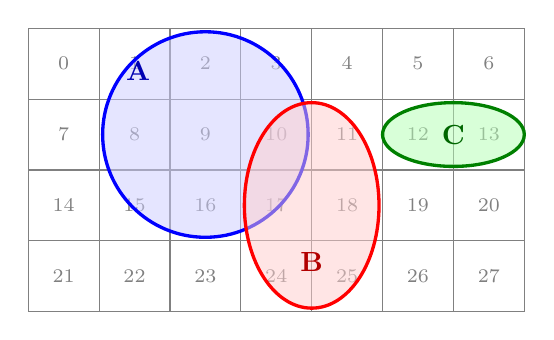
\begin{tikzpicture}[scale=0.9]
\foreach \r in {0,1,2,3}{\foreach \c in {0,...,6}{
 \pgfmathtruncatemacro{\id}{7*\r+\c}
 \draw[gray] (\c,-\r) rectangle (\c+1,-\r-1);
 \node[font=\scriptsize,gray] at (\c+0.5,-\r-0.5) {\id};}}
\draw[blue,very thick,fill=blue!20,fill opacity=0.5] (2.5,-1.5) ellipse (1.45 and 1.45);
\draw[red,very thick,fill=red!20,fill opacity=0.5] (4.0,-2.5) ellipse (0.95 and 1.45);
\draw[green!50!black,very thick,fill=green!30,fill opacity=0.5] (6.0,-1.5) ellipse (1.0 and 0.45);
\node[blue!70!black,font=\bfseries] at (1.55,-0.6) {A};
\node[red!70!black,font=\bfseries] at (4.0,-3.3) {B};
\node[green!40!black,font=\bfseries] at (6.0,-1.5) {C};
\end{tikzpicture}
\caption{$28$ tiles (tile ID $=7\cdot\text{row}+\text{col}$) and three Gaussians A, B, C with view depths $2.1$, $1.4$, $3.0$ (reconstructed from slides 35--36). A touches 9 tiles, B 6 tiles and C 2 tiles: $17$ instances in total.}
\end{figure}

\subsubsection{Tile Rasterizer 2/3: one radix sort \sr{slide 36}}
The instances are generated per Gaussian and per overlapped tile, then sorted once with a radix sort on the 64-bit key.

\begin{center}
\small
\begin{tabular}{@{}lp{11.8cm}@{}}
\toprule
Gaussian & Instances (tile: depth) \\ \midrule
A (2.1) & t1, t2, t3, t8, t9, t10, t15, t16, t17 \\
B (1.4) & t10, t11, t17, t18, t24, t25 \\
C (3.0) & t12, t13 \\ \midrule
\multicolumn{2}{@{}l}{\textbf{After sorting (grouped by tile, front to back inside a tile):}}\\
\multicolumn{2}{@{}p{14.3cm}@{}}{t1:A\ \ t2:A\ \ t3:A\ \ t8:A\ \ t9:A\ \ t10:\textbf{B,A}\ \ t11:B\ \ t12:C\ \ t13:C\ \ t15:A\ \ t16:A\ \ t17:\textbf{B,A}\ \ t18:B\ \ t24:B\ \ t25:B}\\
\bottomrule
\end{tabular}
\end{center}

\begin{proposition}[One global sort gives all per-tile lists]
Sorting instances lexicographically by $(\text{tile ID},\text{depth})$ puts all instances of the same tile in one contiguous block, ordered by increasing depth inside the block.
\end{proposition}
\begin{proof}
The tile ID occupies the high bits, so it is compared first and instances of different tiles are ordered by tile. Within a tile the low bits decide, i.e.\ the depth. (For positive IEEE-754 floats, the integer order of the bit pattern equals the numeric order, so the depth bits can be sorted as integers.)
\end{proof}

\begin{intuition}
It is like sorting a deck of cards by suit first and rank second with one single pass, instead of dealing the cards into four piles and sorting each pile. The GPU then hands each pile (tile) to one block of threads that already knows whom to draw, front to back. The cost is linear in the number $M$ of instances (here $M=17$; in a real scene millions).
\end{intuition}

\begin{remark}[Popping]
Depth is stored \emph{per Gaussian}, not per pixel (slide 36: ``depth per Gaussian, not per pixel $\to$ popping''). Two overlapping, elongated Gaussians may be at the same depth order at one pixel but swapped at another. With a single global order, a small camera motion can flip the centre depths of two Gaussians, and the image changes abruptly (pops).
\end{remark}

\subsubsection{Tile Rasterizer 3/3: Blend Each Tile \sr{slide 37}}
\begin{algorithm}[Per-pixel blending, runs in parallel for every pixel]
\begin{lstlisting}
# runs in parallel for every pixel
def render_pixel(pixel, tile):
    T, C = 1.0, 0.0
    for g in sorted_gaussians[tile]:         # front to back
        d = pixel - g.mean2d
        a = min(0.99, g.opacity
                * exp(-0.5 * d @ inv(g.cov2d) @ d))
        if a < 1 / 255:
            continue                         # too faint
        if T * (1 - a) < 1e-4:
            break                            # pixel saturated
        C += g.color * a * T
        T *= 1 - a
    final_T[pixel] = T                       # kept for backward
    return C
\end{lstlisting}
\end{algorithm}
The four ingredients flagged on the slide: \textbf{front to back} order; \textbf{early stop} when the pixel is saturated; \textbf{skip} $\abar<1/255$; \textbf{clamp} $\abar\le0.99$.

\begin{intuition}
Front to back lets us stop as soon as the pixel is essentially opaque ($T<10^{-4}$): everything behind cannot change the colour. Skipping very faint splats ($<1/255$, below one 8-bit colour level) saves work, and clamping $\abar\le0.99$ guarantees $1-\abar\ge0.01$, so that the backward pass, which divides by $1-\abar$, is numerically safe.
\end{intuition}

\subsection{How to model/aggregate appearance? \sr{slide 38}}
Compute per-Gaussian weights from the opacities of the current and all previous (closer) Gaussians, take the view-dependent colour $\bm c_k$ from the SH coefficients and the ray direction, and aggregate:
\[
w_k=\abar_k\prod_{j=1}^{k-1}(1-\abar_j),\qquad\bm c=\sum_kw_k\bm c_k.
\]

\begin{proposition}[Weights telescope]\label{prop:telescope}
With $T_k=\prod_{j<k}(1-\abar_j)$ we have $w_k=T_k-T_{k+1}$, hence $\sum_{k=1}^Nw_k=1-T_{N+1}\le1$.
\end{proposition}
\begin{proof}
$T_k\abar_k=T_k-T_k(1-\abar_k)=T_k-T_{k+1}$; summing the telescoping series gives $T_1-T_{N+1}=1-T_{N+1}$.
\end{proof}

\begin{example}
For $\abar=(0.5,0.4,0.8)$: $T=(1,0.5,0.3,0.06)$, $w=(0.5,0.2,0.24)$, $\sum w=0.94=1-0.06$. With colours red, green, blue the pixel is $(0.5,0.2,0.24)$, and $6\%$ of the light is left over for whatever is behind (e.g.\ the background colour).
\end{example}

\begin{figure}[htbp]
\centering
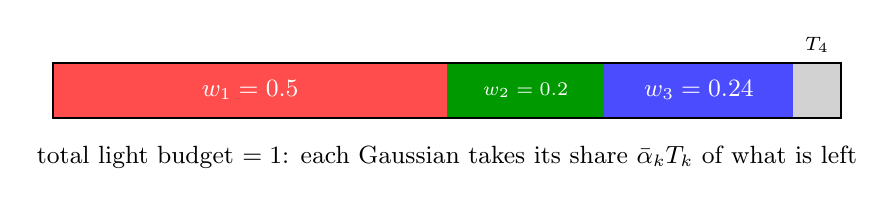
\begin{tikzpicture}
\def\h{0.7}
\fill[red!70] (0,0) rectangle (5.0,\h);\fill[green!60!black] (5.0,0) rectangle (7.0,\h);\fill[blue!70] (7.0,0) rectangle (9.4,\h);\fill[gray!35] (9.4,0) rectangle (10.0,\h);
\draw[thick] (0,0) rectangle (10,\h);
\node[white,font=\small] at (2.5,0.35) {$w_1=0.5$};\node[white,font=\scriptsize] at (6.0,0.35) {$w_2=0.2$};\node[white,font=\small] at (8.2,0.35) {$w_3=0.24$};
\node[font=\scriptsize,anchor=south] at (9.7,\h) {$T_4$};
\node[font=\small] at (5,-0.5) {total light budget $=1$: each Gaussian takes its share $\abar_k T_k$ of what is left};
\end{tikzpicture}
\caption{Light budget of the example: front Gaussians take their share first; later ones only see the transmittance $T_k$ that remains.}
\end{figure}

\begin{intuition}
Think of a pixel as a budget of 1 unit of light. The nearest Gaussian absorbs the fraction $\abar_1$; the next one absorbs $\abar_2$ \emph{of what remains}, and so on. This is exactly the volume-rendering bookkeeping $T_i\alpha_i$ of the recap, with $\abar_k$ playing the role of $\alpha_i$, but evaluated only at the primitives instead of at many empty samples.
\end{intuition}
%=====================================================================
\section{3D Gaussian Splatting: The Full Pipeline \sr{slides 39--41}}
%=====================================================================
\subsection{The Full Pipeline \sr{slide 39}}
\begin{itemize}[nosep]
\item \textbf{Forward:} project $\to$ sort $\to$ blend.
\item \textbf{Backward:} gradients to every Gaussian.
\item \textbf{Density control:} add and remove Gaussians.
\end{itemize}

\begin{figure}[htbp]
\centering
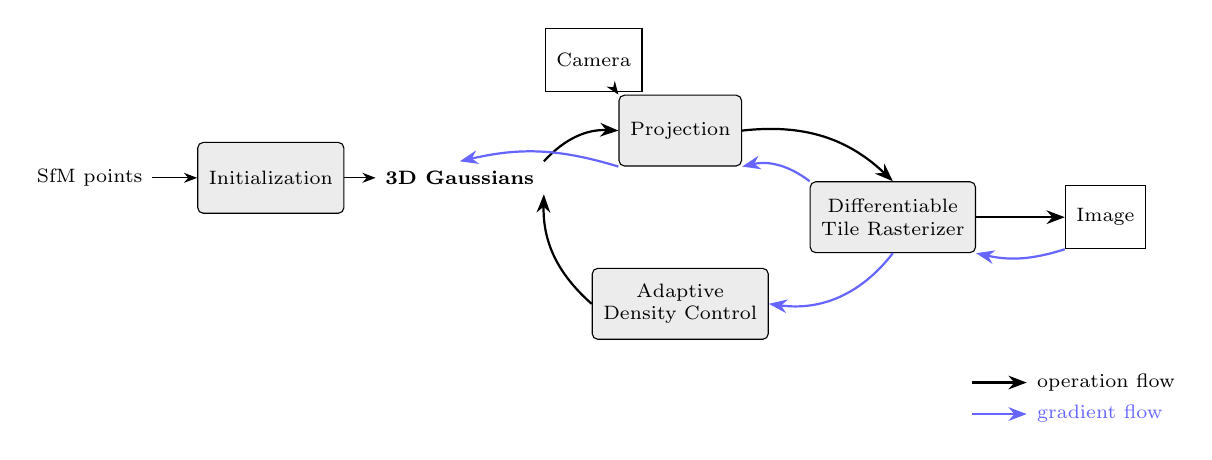
\begin{tikzpicture}[blk/.style={draw,rounded corners=2pt,fill=gray!15,align=center,font=\scriptsize,minimum height=0.9cm,inner sep=4pt},
 io/.style={draw,align=center,font=\scriptsize,minimum height=0.8cm,inner sep=4pt},>={Stealth}]
\node[font=\scriptsize,align=center] (sfm) at (0,0) {SfM points};
\node[blk] (init) at (2.3,0) {Initialization};
\node[font=\scriptsize,align=center] (g) at (4.7,0) {\textbf{3D Gaussians}};
\node[io] (cam) at (6.4,1.5) {Camera};
\node[blk] (proj) at (7.5,0.6) {Projection};
\node[blk] (ras) at (10.2,-0.5) {Differentiable\\Tile Rasterizer};
\node[io] (img) at (12.9,-0.5) {Image};
\node[blk] (adc) at (7.5,-1.6) {Adaptive\\Density Control};
\draw[->] (sfm)--(init); \draw[->] (init)--(g);
\draw[->,thick] (g.north east) to[bend left=25] (proj.west);
\draw[->] (cam)--(proj.north west);
\draw[->,thick] (proj.east) to[bend left=25] (ras.north);
\draw[->,thick] (ras)--(img);
\draw[->,thick] (adc.west) to[bend left=25] (g.south east);
\draw[->,blue!60,thick] (proj.south west) to[bend right=15] (g.north);
\draw[->,blue!60,thick] (ras.north west) to[bend right=25] (proj.south east);
\draw[->,blue!60,thick] (ras.south) to[bend left=30] (adc.east);
\draw[->,blue!60,thick] (img.south west) to[bend left=15] (ras.south east);
\draw[->,thick] (11.2,-2.6)--(11.9,-2.6) node[right,font=\scriptsize] {operation flow};
\draw[->,blue!60,thick] (11.2,-3.0)--(11.9,-3.0) node[right,font=\scriptsize] {gradient flow};
\end{tikzpicture}
\caption{The 3DGS pipeline (Kerbl et al., SIGGRAPH 2023), redrawn from slide 39. Black arrows: operation flow; blue arrows: gradient flow. Gradients from the rasterizer reach the projection (and hence the Gaussian parameters) and also drive the adaptive density control.}
\end{figure}

\subsection{Backward Pass: Gradients Through Blending \sr{slide 40}}
Let $\bm c=\sum_{i=1}^N\bm c_i\,\abar_i\,T_i$ with $T_i=\prod_{j<i}(1-\abar_j)$.

\begin{proposition}[Gradients of front-to-back blending]\label{prop:bwd}
\[
\frac{\partial\bm c}{\partial\bm c_i}=\abar_iT_i,\qquad
\frac{\partial\bm c}{\partial\abar_i}=T_i\bm c_i-\frac{1}{1-\abar_i}\sum_{j>i}\bm c_j\abar_jT_j .
\]
\end{proposition}
\begin{proof}
$\bm c_i$ appears only in term $i$, with coefficient $\abar_iT_i$. The opacity $\abar_i$ appears (a) in term $i$ as the factor $\abar_i$, giving $T_i\bm c_i$ (because $T_i$ does not depend on $\abar_i$), and (b) inside $T_j$ for every $j>i$ through the factor $(1-\abar_i)$, so $\partial T_j/\partial\abar_i=-T_j/(1-\abar_i)$, contributing $-\sum_{j>i}\bm c_j\abar_jT_j/(1-\abar_i)$.
\end{proof}

\begin{algorithm}[Backward pass: walk back to front, recover $T$ from the final $T$]\label{alg:bwd}
Since $T_{i+1}=T_i(1-\abar_i)$ we get $T_i=T_{i+1}/(1-\abar_i)$. Only the final transmittance $T_{N+1}$ (\texttt{final\_T}) must be stored in the forward pass. With upstream gradient $\bm g=\partial\Lc/\partial\bm c$:
\begin{lstlisting}
T = final_T[pixel];  S = 0              # S = sum_{j>i} c_j a_j T_j
for i in reversed(range(N)):            # back to front
    T = T / (1 - a[i])                  # now T = T_i
    grad_c[i] = a[i] * T * g
    grad_a[i] = g @ (T * c[i] - S / (1 - a[i]))
    S += c[i] * a[i] * T
\end{lstlisting}
\end{algorithm}

\begin{example}
Scalar colours $c=(1,0.5,1)$, $\abar=(0.5,0.4,0.8)$, so $T=(1,0.5,0.3)$. Then $\partial c/\partial\abar_2=T_2c_2-\frac1{1-0.4}c_3\abar_3T_3=0.25-\frac{0.24}{0.6}=-0.15$. Directly: $c=0.9-0.15\,\abar_2$, whose derivative is $-0.15$. $\checkmark$
\end{example}

\begin{intuition}
The two terms in $\partial\bm c/\partial\abar_i$ are a tug of war. Making Gaussian $i$ more opaque (1) adds more of its \emph{own} colour (positive term $T_i\bm c_i$), but (2) hides everything behind it (negative term, the colour that would have come from behind). Whether the net effect is positive depends on whether $\bm c_i$ is brighter or darker (relative to the loss) than the stuff behind. Walking back to front lets us accumulate ``the stuff behind'' in the running sum $S$ with no per-sample storage; the clamp $\abar\le0.99$ makes the division safe.
\end{intuition}

The upstream gradient $\partial\Lc/\partial\abar_i$ is then propagated through $\abar_i=\alpha_i\exp(\cdot)$ to $\alpha_i$, $\bm\mu_{2D}$ and $\bm\Sigma_{2D}$, and through the projection ($\bm J$, $\bm W$) and the factorisation to $\bm\mu,\bm s,\bm q$; the SH coefficients receive $\partial\bm c/\partial\bm c_i$.

\subsection{Optimization \sr{slide 41}}
The loss mixes an $\ell_1$ term and a structural term, $\Lc=(1-\lambda)\Lc_1+\lambda\Lc_{\text{D-SSIM}}$ with $\lambda=0.2$. Training runs for 30K iterations of Adam, one full image per step, with per-parameter learning rates:
\begin{center}
\begin{tabular}{@{}ll@{}}
\toprule
Parameter & Learning rate \\ \midrule
position $\bm\mu$ & $1.6\cdot10^{-4}\to1.6\cdot10^{-6}$ \\
SH coefficients & $2.5\cdot10^{-3}$ \\
opacity & $2.5\cdot10^{-2}$ \\
scale & $5\cdot10^{-3}$ \\
rotation & $10^{-3}$ \\ \bottomrule
\end{tabular}
\end{center}

\begin{intuition}
Different parameters live on different scales, so one learning rate does not fit all: opacity (a number in $(0,1)$) can move fast, while positions are in scene units and must settle gently, hence the decay by a factor 100 over training.
\end{intuition}

%=====================================================================
\section{Initialization, Densification and Ablations \sr{slides 42--45}}
%=====================================================================
\subsection{Initialization: SfM Points vs Random \sr{slide 42}}
\begin{itemize}[nosep]
\item One Gaussian per SfM point.
\item Isotropic, $\alpha=0.1$.
\item Random initialization gives a worse background.
\end{itemize}
\slideimage[5.0cm]{42}{Garden scene: random initialization (top row) vs.\ SfM initialization (bottom row) and a zoomed crop; the random init is visibly worse in the background. From Kerbl et al., 2023.}

\subsection{Adaptive Density Control \sr{slide 43}}
Triggered by \textbf{large positional gradients}:
\begin{itemize}[nosep]
\item \textbf{Small} Gaussian: \emph{clone}.
\item \textbf{Large} Gaussian: \emph{split}, scale $\div1.6$.
\item \textbf{Prune} $\alpha<0.005$.
\item \textbf{Reset} $\alpha$ every 3000 iterations.
\end{itemize}

\begin{algorithm}[Adaptive density control]
For each Gaussian whose accumulated view-space positional gradient exceeds a threshold: if it is small, clone it (copy, then let optimisation separate the two); if it is large, replace it by two Gaussians with scales divided by $1.6$. Remove Gaussians with $\alpha<0.005$. Every 3000 iterations, reset all opacities to a low value.
\end{algorithm}

\begin{remark}[Beyond the slides]
In Kerbl et al.\ the positional-gradient threshold is $\tau_{pos}=2\cdot10^{-4}$, densification runs every 100 iterations until about iteration 15K, and the two Gaussians of a split are placed by sampling positions from the original Gaussian. Resetting opacity lets Gaussians that are really needed regain opacity within a few iterations while floaters stay transparent and are pruned.
\end{remark}

\begin{figure}[htbp]
\centering
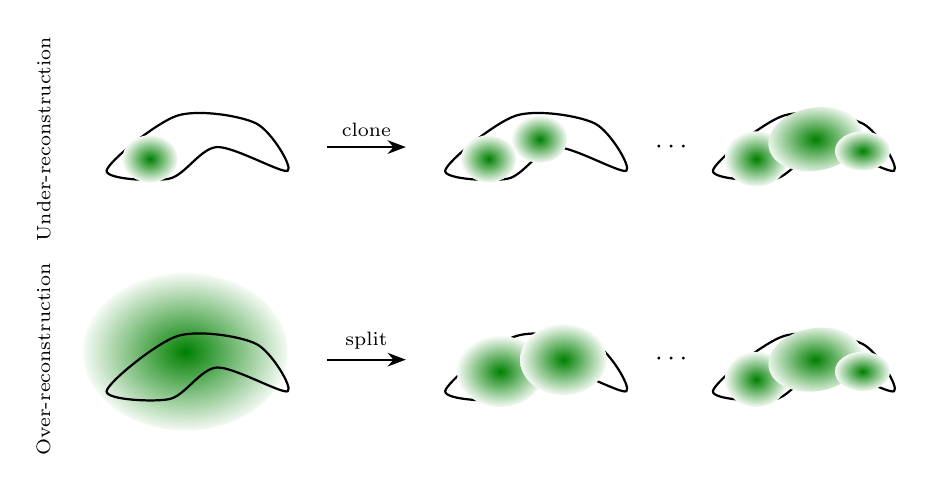
\begin{tikzpicture}[>={Stealth}]
\def\bean{plot[smooth cycle] coordinates {(0,0.2) (0.9,0.9) (1.9,0.8) (2.3,0.2) (1.4,0.5) (0.8,0.1)}}
% under-reconstruction
\node[font=\scriptsize,rotate=90] at (-0.8,0.6) {Under-reconstruction};
\draw[thick,fill=white] \bean;
\blob{0.55}{0.35}{0.35}{0.3}{0}{green!50!black}
\draw[->,thick] (2.8,0.5)--(3.8,0.5) node[midway,above,font=\scriptsize] {clone};
\begin{scope}[xshift=4.3cm]
\draw[thick,fill=white] \bean;
\blob{0.55}{0.35}{0.35}{0.3}{0}{green!50!black}\blob{1.2}{0.6}{0.35}{0.3}{0}{green!50!black}
\end{scope}
\node at (7.2,0.5) {$\cdots$};
\begin{scope}[xshift=7.7cm]
\draw[thick,fill=white] \bean;
\blob{0.55}{0.35}{0.4}{0.35}{0}{green!50!black}\blob{1.3}{0.6}{0.6}{0.4}{10}{green!50!black}\blob{1.9}{0.45}{0.35}{0.25}{0}{green!50!black}
\end{scope}
% over-reconstruction
\node[font=\scriptsize,rotate=90] at (-0.8,-2.2) {Over-reconstruction};
\begin{scope}[yshift=-2.8cm]
\blob{1.0}{0.7}{1.3}{1.0}{0}{green!50!black}
\draw[thick] \bean;
\end{scope}
\draw[->,thick] (2.8,-2.2)--(3.8,-2.2) node[midway,above,font=\scriptsize] {split};
\begin{scope}[xshift=4.3cm,yshift=-2.8cm]
\draw[thick,fill=white] \bean;
\blob{0.7}{0.45}{0.55}{0.45}{0}{green!50!black}\blob{1.5}{0.6}{0.55}{0.45}{0}{green!50!black}
\end{scope}
\node at (7.2,-2.2) {$\cdots$};
\begin{scope}[xshift=7.7cm,yshift=-2.8cm]
\draw[thick,fill=white] \bean;
\blob{0.55}{0.35}{0.4}{0.35}{0}{green!50!black}\blob{1.3}{0.6}{0.6}{0.4}{10}{green!50!black}\blob{1.9}{0.45}{0.35}{0.25}{0}{green!50!black}
\end{scope}
\end{tikzpicture}
\caption{Adaptive density control (redrawn from slide 43): a too small Gaussian that does not cover the shape is cloned; a too large Gaussian that blurs the shape is split into smaller ones. Optimisation then continues.}
\end{figure}

\begin{intuition}
A large positional gradient means ``many pixels disagree about where this Gaussian should be'': it is trying to be in several places at once. If it is already small, the geometry is simply under-covered, so we add a copy (clone). If it is big, one blob is trying to explain structure that needs detail, so we replace it by smaller ones (split, $\div1.6$ in scale). Pruning removes Gaussians that contribute almost nothing.
\end{intuition}

\subsection{Ablation: Densification \sr{slide 44}}
\slideimage[3.6cm]{44}{Bicycle crop, three versions: \textbf{No split} (blurry background), \textbf{No clone} (broken spokes, the arrow marks the wheel), \textbf{Full}. From Kerbl et al., 2023.}
Without splitting, large Gaussians cannot be refined and the background stays blurry; without cloning, thin structures such as spokes are not covered by enough Gaussians.

\subsection{Ablation: Anisotropy \sr{slide 45}}
\slideimage[3.8cm]{45}{Potted plant: ground truth, full model (anisotropic Gaussians) and the isotropic ablation, which yields blobs instead of leaves. From Kerbl et al., 2023.}

\begin{figure}[htbp]
\centering
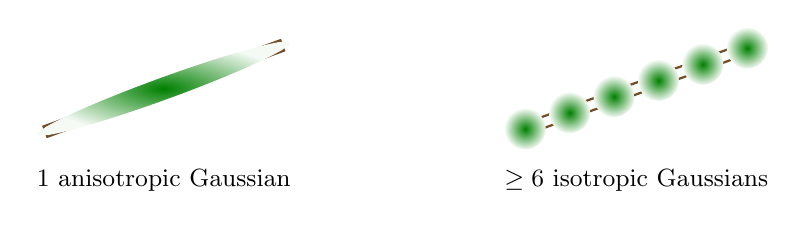
\begin{tikzpicture}
\begin{scope}
\draw[brown!60!black,thick,rotate=20] (-1.6,-0.07) rectangle (1.6,0.07);
\blob{0}{0}{1.7}{0.14}{20}{green!50!black}
\node[font=\small,below] at (0,-0.9) {1 anisotropic Gaussian};
\end{scope}
\begin{scope}[xshift=6cm]
\draw[brown!60!black,thick,rotate=20] (-1.6,-0.07) rectangle (1.6,0.07);
\foreach \t in {-1.5,-0.9,-0.3,0.3,0.9,1.5}{\blob{{\t*cos(20)}}{{\t*sin(20)}}{0.26}{0.26}{0}{green!50!black}}
\node[font=\small,below] at (0,-0.9) {$\ge6$ isotropic Gaussians};
\end{scope}
\end{tikzpicture}
\caption{Toy example (not on the slides): a thin leaf or branch needs a single stretched ellipsoid, but a chain of many round blobs if only isotropic Gaussians are allowed, and the result still looks dotted.}
\end{figure}

\begin{intuition}
Natural scenes are full of thin or flat things (leaves, spokes, walls). An anisotropic Gaussian is a pencil or a sheet of paint; an isotropic one is a ball. Using balls to draw lines needs many more balls and leaves visible beads, as seen in the plant ablation.
\end{intuition}

%=====================================================================
\section{Results: Quality and Speed \sr{slides 46--48}}
%=====================================================================
\begin{center}
\small
\begin{tabular}{@{}lccccrr@{}}
\toprule
Method & PSNR$\uparrow$ & SSIM$\uparrow$ & LPIPS$\downarrow$ & Train & FPS & Memory \\ \midrule
Plenoxels & 23.08 & 0.626 & 0.463 & 25m49s & 6.8 & 2.1 GB \\
Instant-NGP (big) & 25.59 & 0.699 & 0.331 & 7m30s & 9.4 & 48 MB \\
Mip-NeRF360 & 27.69 & 0.792 & 0.237 & 48 h & 0.06 & 8.6 MB \\
3DGS, 7K iter. & 25.60 & 0.770 & 0.279 & 6m25s & 160 & 523 MB \\
3DGS, 30K iter. & 27.21 & 0.815 & 0.214 & 41m33s & 134 & 734 MB \\ \bottomrule
\end{tabular}

\smallskip
{\footnotesize Kerbl et al., SIGGRAPH 2023, Table 1 (Mip-NeRF360 dataset).}
\end{center}

\begin{example}[Reading the table]
Against Mip-NeRF360, 3DGS (30K) loses $0.48$~dB of PSNR but has better SSIM and LPIPS, trains $\approx69\times$ faster ($2880$~min vs.\ $41.5$~min) and renders $\approx2200\times$ faster ($134$ vs.\ $0.06$~FPS). The price is memory: $734$~MB vs.\ $8.6$~MB, about $85\times$. After only 7K iterations (6.5~min) 3DGS already matches Instant-NGP's PSNR with an order of magnitude higher frame rate.
\end{example}

\begin{intuition}
NeRF-type models store the scene in a small network and pay at render time (many network queries per ray). 3DGS stores the scene explicitly (millions of Gaussians) and pays in memory, but rendering is just ``splat and blend'', which GPUs do extremely well. It trades memory for speed.
\end{intuition}

\slideimage[4.4cm]{47}{Interactive 3DGS viewer on the bicycle scene, showing 57.56 FPS (17.37 ms) with VSync on.}
\slideimage[4.4cm]{48}{Interactive 3DGS viewer on an indoor playroom scene, showing 89.37 FPS (11.19 ms).}

%=====================================================================
\section{Limitations \sr{slide 49}}
%=====================================================================
\slideimage[3.6cm]{49}{Mip-NeRF360 (left) vs.\ 3DGS (right) on a train scene: 3DGS reconstructs the foreground structures that Mip-NeRF360 smears.}
\begin{itemize}
\item \textbf{Memory:} millions of Gaussians (hundreds of MB per scene).
\item \textbf{Popping:} the per-Gaussian sort (Remark in the Tile Rasterizer 2/3 subsection).
\item \textbf{Aliasing under zoom} $\to$ Mip-Splatting.
\item \textbf{No surfaces} $\to$ SuGaR, 2DGS.
\end{itemize}
\begin{intuition}
Each limitation is a consequence of a design choice. Explicit storage costs memory. A global depth order per Gaussian is cheap but only approximately correct. A fixed-size screen-space filter does not adapt when zooming. And a volumetric blob has no well-defined surface or normal. The next section shows how swapping the primitive addresses the last one.
\end{intuition}

%=====================================================================
\section{Other Primitives \sr{slides 50--54}}
%=====================================================================
\subsection{Other Primitives: Fuzzy Metaballs \sr{slide 50}}
Keselman and Hebert, \emph{Fuzzy Metaballs: Approximate Differentiable Rendering with Algebraic Surfaces}, ECCV 2022 (Oral). The slide shows a teddy bear fitted from a target mask: the estimated mask and depth start as a small cloud at iteration 0 and are optimised towards the target.
\slideimage[4.4cm]{50}{Fuzzy Metaballs optimisation on a teddy bear: input photo, target mask, estimated mask and estimated depth at iteration 0 (epoch 0.0).}

\subsection{2D Gaussian Splatting: The Primitive \sr{slide 51}}
Huang et al., SIGGRAPH 2024. A 3D Gaussian intersected by a plane gives different cross-sections for different viewpoints, whereas a 2D Gaussian is a flat disc whose intersection with every viewing ray is well defined and view-consistent.

\begin{figure}[htbp]
\centering
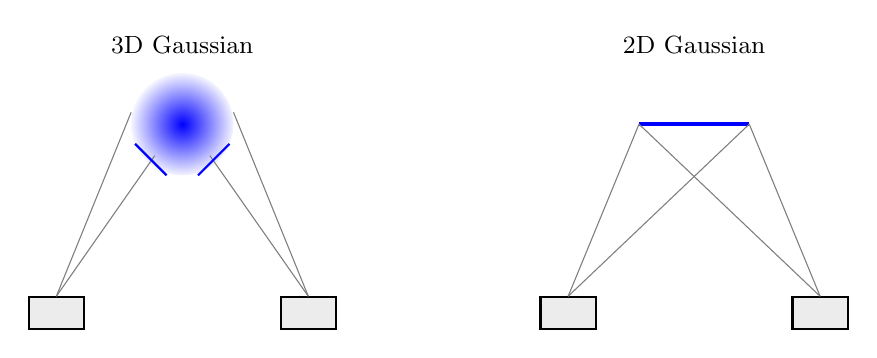
\begin{tikzpicture}[cam/.style={draw,thick,fill=gray!15,minimum width=0.7cm,minimum height=0.4cm,inner sep=0pt}]
\node[font=\small] at (1.6,3.4) {3D Gaussian};
\blob{1.6}{2.4}{0.65}{0.65}{0}{blue}
\node[cam] (c1) at (0,0) {}; \node[cam] (c2) at (3.2,0) {};
\draw[gray] (c1.north)--(1.25,2.0); \draw[gray] (c1.north)--(0.95,2.55);
\draw[gray] (c2.north)--(1.95,2.0); \draw[gray] (c2.north)--(2.25,2.55);
\draw[thick,blue] (1.0,2.15) -- (1.4,1.75); \draw[thick,blue] (2.2,2.15)--(1.8,1.75);
\begin{scope}[xshift=6.5cm]
\node[font=\small] at (1.6,3.4) {2D Gaussian};
\draw[very thick,blue] (0.9,2.4)--(2.3,2.4);
\node[cam] (d1) at (0,0) {}; \node[cam] (d2) at (3.2,0) {};
\draw[gray] (d1.north)--(0.9,2.4); \draw[gray] (d1.north)--(2.3,2.4);
\draw[gray] (d2.north)--(0.9,2.4); \draw[gray] (d2.north)--(2.3,2.4);
\end{scope}
\end{tikzpicture}
\caption{Left: a 3D Gaussian is intersected by planes that differ per viewpoint. Right: a 2D Gaussian is the same planar disc for every camera (schematic, after slide 51).}
\end{figure}

\begin{definition}[2D Gaussian splat]
A splat has a centre $\bm p_k$, two tangent vectors $\bm t_u,\bm t_v$ with scales $s_u,s_v$, and lives in its own tangent plane:
\[
P(u,v)=\bm p_k+s_u\bm t_u\,u+s_v\bm t_v\,v=\bm H\,(u,v,1,1)\T,\qquad
\bm H=\begin{bmatrix}\bm R\bm S&\bm p_k\\\bm 0\T&1\end{bmatrix},
\]
with $\bm R=[\bm t_u\ \bm t_v\ \bm t_w]$ and $\G(u,v)=\exp\!\big(-\tfrac{u^2+v^2}{2}\big)$. The splat is \textbf{flat}: $\bm S=\diag(s_u,s_v,0)$; its \textbf{normal} is $\bm t_w=\bm t_u\times\bm t_v$.
\end{definition}

\begin{intuition}
A 2D Gaussian is a fuzzy coin instead of a fuzzy ball. A coin has a definite orientation (its normal), and one ray hits it at one point, so a single hit gives an \textbf{exact depth}. A ball only gives a smeared volumetric depth.
\end{intuition}

\subsection{2D Gaussian Splatting: Ray-Splat Intersection \sr{slide 52}}
\begin{enumerate}
\item \textbf{A pixel is two planes.} The ray through pixel $(x,y)$ is the intersection of the $x$-plane $\bm h_x=(-1,0,0,x)\T$ and the $y$-plane $\bm h_y=(0,-1,0,y)\T$.
\item \textbf{Move the planes to the splat frame without an inverse:} $\bm h_u=(\bm W\bm H)\T\bm h_x$, $\bm h_v=(\bm W\bm H)\T\bm h_y$.
\item \textbf{Solve for $(u,v)$:} $\bm h_u\cdot(u,v,1,1)\T=\bm h_v\cdot(u,v,1,1)\T=0$.
\item \textbf{Edge-on case:} use a screen-space floor, $\hat\G(\bm x)=\max\{\G(\bm u(\bm x)),\ \G(\tfrac{\bm x-\bm c}{\sigma})\}$.
\end{enumerate}
Then proceed as in 3DGS: tiles, sort and blend.

\begin{proposition}[Closed-form ray--splat hit]
Because the third column of $\bm H$ is zero ($s_w=0$), the third component of $\bm h_u,\bm h_v$ vanishes and the system in step 3 reads $h_u^1u+h_u^2v+h_u^4=0$, $h_v^1u+h_v^2v+h_v^4=0$, with solution
\[
u=\frac{h_u^2h_v^4-h_u^4h_v^2}{h_u^1h_v^2-h_u^2h_v^1},\qquad
v=\frac{h_u^4h_v^1-h_u^1h_v^4}{h_u^1h_v^2-h_u^2h_v^1}.
\]
\end{proposition}
\begin{proof}
Cramer's rule on the $2\times2$ system. The denominator vanishes exactly when the splat is seen edge-on (the ray is parallel to the splat's plane), which is the degenerate case handled by the floor in step 4.
\end{proof}

\begin{intuition}
Two planes (``everything with this $x$'' and ``everything with this $y$'') meet in a line, which is the pixel's ray. Pushing both planes into the splat's own coordinates lets us read off the hit $(u,v)$ by solving two linear equations: no matrix inversion, and the Gaussian weight at the hit is $\G(u,v)$ exactly, rather than a projected approximation. When the coin is seen edge-on it has no area on screen, so we keep a small blob of fixed screen size to avoid losing it (and its gradients).
\end{intuition}

\subsection{From Cameras to LiDAR: Splat-LOAM \sr{slide 53}}
Giacomini, Di Giammarino, De Rebotti, Grisetti and Oswald, ICCV 2025. The pipeline: a \textbf{LiDAR scan $\to$ range image}; a \textbf{spherical 2DGS rasterizer}; \textbf{range-only supervision}; \textbf{map + odometry}.

\begin{figure}[htbp]
\centering
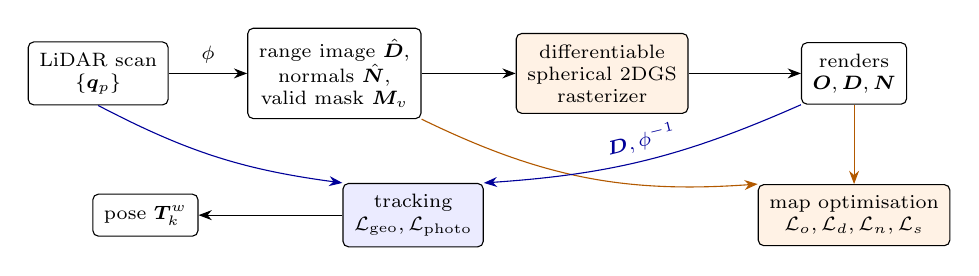
\begin{tikzpicture}[blk/.style={draw,rounded corners=2pt,align=center,font=\scriptsize,fill=white,inner sep=4pt},>={Stealth}]
\node[blk] (scan) at (0,0) {LiDAR scan\\$\{\bm q_p\}$};
\node[blk] (img) at (3.0,0) {range image $\hat{\bm D}$,\\normals $\hat{\bm N}$,\\valid mask $\bm M_v$};
\node[blk,fill=orange!10] (ras) at (6.4,0) {differentiable\\spherical 2DGS\\rasterizer};
\node[blk] (out) at (9.6,0) {renders\\$\bm O,\bm D,\bm N$};
\node[blk,fill=orange!10] (map) at (9.6,-1.8) {map optimisation\\$\Lc_o,\Lc_d,\Lc_n,\Lc_s$};
\node[blk,fill=blue!8] (trk) at (4.0,-1.8) {tracking\\$\Lc_{\text{geo}},\Lc_{\text{photo}}$};
\node[blk] (pose) at (0.6,-1.8) {pose $\bm T^w_k$};
\draw[->] (scan)--node[above,font=\scriptsize]{$\phi$}(img);
\draw[->] (img)--(ras); \draw[->] (ras)--(out);
\draw[->,orange!70!black] (out)--(map); \draw[->,orange!70!black] (img.south east) to[bend right=15] (map.north west);
\draw[->,blue!60!black] (out.south west) to[bend left=10] node[above,font=\scriptsize,sloped]{$\bm D,\phi^{-1}$}(trk.north east);
\draw[->,blue!60!black] (scan.south) to[bend right=10] (trk.north west);
\draw[->] (trk)--(pose);
\end{tikzpicture}
\caption{Splat-LOAM, schematically redrawn from slide 53 (block names from the slide; the exact loss definitions are in the paper). The map is optimised from range images, while tracking estimates the sensor pose $\bm T_k^w$ against the rendered depth.}
\end{figure}

\begin{example}[Spherical projection to a range image]
A LiDAR point $\bm q=(x,y,z)$ has range $r=\|\bm q\|$, azimuth $\theta=\operatorname{atan2}(y,x)$ and elevation $\varphi=\arcsin(z/r)$. A range image stores $\bm D(u,v)=r$ at $u\propto\theta$, $v\propto\varphi$ (the standard spherical camera model, not detailed on the slide).
\end{example}
\slideimage[4.4cm]{53}{Splat-LOAM results panel: the rendered normal map of the reconstructed building (right part of the figure).}

\subsection{Beyond Gaussians: Other Primitives \sr{slide 54}}
\begin{itemize}[nosep]
\item \textbf{Voxels:} SVRaster (Sun et al., CVPR 2025).
\item \textbf{Triangles:} Triangle Splatting (Held et al., 2025).
\item \textbf{Voronoi cells:} Radiant Foam (Govindarajan et al., 2025).
\end{itemize}
\slideimage[5.0cm]{54}{Three alternative primitives on the garden scene: sparse voxels (SVRaster), triangles (Triangle Splatting) and Voronoi cells (Radiant Foam).}

\begin{intuition}
The recipe of this lecture stays fixed: (1) find the primitives that touch a pixel (project and bin them into tiles), (2) order them, (3) blend front to back. What changes from primitive to primitive is only the \emph{footprint} (ellipse, coin, triangle with soft edge, box, polygonal cell) and how its opacity falls off, so that the whole pipeline remains differentiable.
\end{intuition}

%=====================================================================
\section{Summary \sr{slide 55}}
%=====================================================================
\textbf{Rasterization + blending for efficient rendering.} \textbf{Aggregating `soft' primitives along a ray allows differentiable rendering.} \textbf{Projecting 3D Gaussians gives 2D rendering} via $\bm\mu_{2D}=\pi(\bm\mu_{3D})$, $\bm\Sigma_{2D}=\bm J\bm\Sigma_{3D}\bm J\T$.

\begin{center}
\small
\renewcommand{\arraystretch}{1.25}
\begin{tabularx}{\linewidth}{@{}p{2.45cm}p{2.3cm}XX@{}}
\toprule
Method & Primitive & How it renders / stays differentiable & Main limitation \\ \midrule
Hard mesh ray-casting & triangles & closest hit per ray; $(\alpha,\beta)$ smooth in vertices & jumps at occlusion and depth order; no gradient to hidden faces \\
Soft Rasterizer / PyTorch3D & soft triangles & sigmoid mask of pixel distance + $K$ closest, depth-softmax weights; primitive-major loop & blur controlled by $\sigma,\gamma$; only $K$ layers \\
3D Gaussian Splatting & 3D Gaussians & EWA projection $\bm J\bm\Sigma\bm J\T$; one radix sort on (tile, depth); front-to-back $\alpha$-blending with analytic backward & memory, popping, aliasing, no surface \\
2D Gaussian Splatting & flat Gaussians (discs) & exact ray--splat intersection in splat frame; exact depth and normal & edge-on views need a screen-space floor \\
Splat-LOAM & spherical 2DGS & range-image rasterizer, range-only supervision, map + odometry & LiDAR only (no appearance) \\
Other & voxels, triangles, Voronoi cells & same project--sort--blend skeleton with another footprint & see papers \\ \bottomrule
\end{tabularx}
\end{center}

\begin{figure}[htbp]
\centering
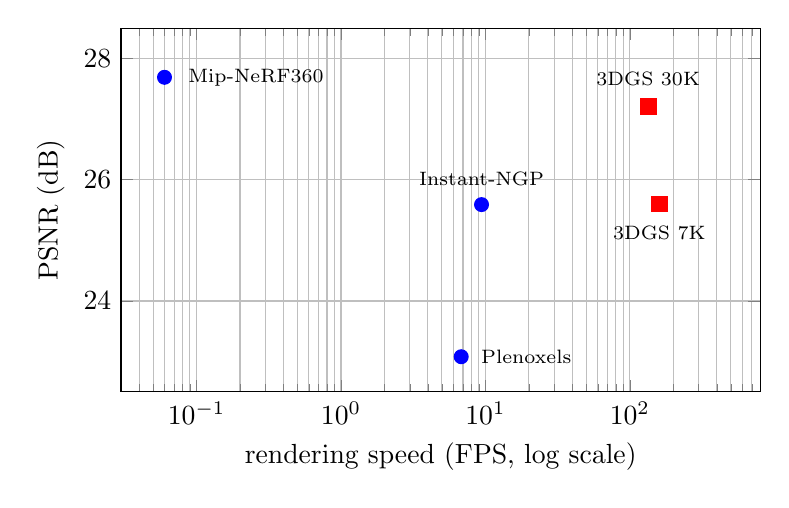
\begin{tikzpicture}
\begin{axis}[width=0.8\linewidth,height=6.2cm,xmode=log,xlabel={rendering speed (FPS, log scale)},ylabel={PSNR (dB)},
 xmin=0.03,xmax=800,ymin=22.5,ymax=28.5,grid=both,clip=false]
\addplot[only marks,mark=*,mark size=2.5pt,blue] coordinates {(6.8,23.08) (9.4,25.59) (0.06,27.69)};
\addplot[only marks,mark=square*,mark size=2.8pt,red] coordinates {(160,25.60) (134,27.21)};
\node[anchor=west,font=\scriptsize] at (axis cs:8,23.08) {Plenoxels};
\node[anchor=south,font=\scriptsize] at (axis cs:9.4,25.75) {Instant-NGP};
\node[anchor=west,font=\scriptsize] at (axis cs:0.075,27.69) {Mip-NeRF360};
\node[anchor=north,font=\scriptsize] at (axis cs:160,25.4) {3DGS 7K};
\node[anchor=south,font=\scriptsize] at (axis cs:134,27.4) {3DGS 30K};
\end{axis}
\end{tikzpicture}
\caption{Quality vs.\ speed on Mip-NeRF360 (data from the results table): the 3DGS points (red) sit towards the top right, i.e.\ near-best quality at real-time rates.}
\end{figure}

\subsection*{Key take-aways}
\begin{enumerate}
\item \textbf{Primitive rendering = find influencing primitives + aggregate.} Unlike volume rendering it does not waste samples in empty space.
\item \textbf{Hard rendering is not differentiable where it matters:} occlusion and depth ordering create jumps. Soft masks (sigmoid of signed distance) and depth-softmax blending turn the jumps into smooth transitions and give gradients to hidden primitives.
\item \textbf{Rasterization swaps the loop order} (primitives first, pixels second), replacing $\Theta(PN)$ tests by $\Theta(N\bar f+PK)$; 3DGS does it with tiles and a single radix sort on (tile ID, depth).
\item \textbf{3DGS in three formulas:} $\bm\Sigma=\bm R\bm S\bm S\T\bm R\T$ (always PSD), $\bm\Sigma_{2D}=\bm J\bm W\bm\Sigma\bm W\T\bm J\T$ (EWA), and front-to-back blending $\bm c=\sum_k\bm c_k\abar_kT_k$ with a back-to-front analytic gradient that only needs the final transmittance.
\item \textbf{Optimisation is more than gradient descent:} adaptive density control (clone, split, prune, opacity reset) and SfM initialisation are essential; limitations (memory, popping, aliasing, no surfaces) motivate Mip-Splatting, 2DGS, SuGaR and other primitives.
\end{enumerate}

\bigskip
\textbf{Acknowledgments (slide 56).} The slides are adapted from \emph{Learning for 3D Vision}, CMU 16-825 (Prof.\ Shubham Tulsiani); the Gaussian-representation slide is adapted from Vincent Sitzmann. Results and diagrams are from Ravi et al.\ 2020 (PyTorch3D), Liu et al.\ ICCV 2019 (Soft Rasterizer), Zwicker et al.\ 2001 (EWA Volume Splatting), Kerbl et al.\ SIGGRAPH 2023 (3D Gaussian Splatting), Keselman and Hebert ECCV 2022 (Fuzzy Metaballs), Huang et al.\ SIGGRAPH 2024 (2D Gaussian Splatting), Giacomini et al.\ ICCV 2025 (Splat-LOAM), Sun et al.\ CVPR 2025 (SVRaster), Held et al.\ 2025 (Triangle Splatting) and Govindarajan et al.\ 2025 (Radiant Foam).

\end{document}
